\chapter{Artificial Neural Networks for EHL Film Thickness Predictions}
\label{ANN Lubricated Bearing FMBD}

\section{Introduction}

Tribodynamic modelling generally employs analytical equations for the prediction of film thickness in elastohydrodynamic contacts; chosen due to their timely solution. Whilst computationally efficient, these do not achieve the accuracy of the full numerical solution outside the bounds of the data used to generate the analytical equations. In the context of dynamic simulation, a full numerical solution at each time step of a system level model would, however, yield excessive computation time. This has led to the emerging use of data driven solutions, such as machine learning, in the field of tribology. These can achieve accuracy much closer to the numerical solution, whilst significantly improving computational time.

This chapter details the development of an Artificial Neural Network (ANN) for prediction of central film thickness at the roller-race conjunction. ANNs are trained using data generated by the numerical EHL solution, with the data set constrained to realistic operating conditions using the Greenwood regimes of lubrication. Multiple ANNs are compared to find the optimum structure, accounting for training time and accuracy. The ANN is then deployed explicitly, using the boundary conditions of a simple bearing model to test the film thickness accuracy and speed of solution. The trained ANN is then deployed implicitly in the system level FMBD introduced in Chapter \ref{Lubricated FMBD}, replacing the analytical film equations in the model.

The aim of this chapter is to improve the accuracy of the central film thickness estimation, whilst maintaining a timely solution in the context of a full dynamic solution. This workflow employed is not only relevant to roller bearings; it can be applied to a wide range of contacts and different sources of training data depending on the modelling requirements.

\section{Numerical vs Analytical Film Thickness Estimations at High Entrainment Velocities}

Two main approaches exist for determination of the complex non-linear problem of film thickness in lubricated contacts. The first approach involves employing numerical methods \cite{Dowson1959}, where systems of partial differential equations are formulated to describe the state of the contact and then solved iteratively \cite{Gohar2018}. While this method yields accurate results and is applicable to a wide range of operating conditions, it is computationally intensive due to its iterative nature. The second approach involves developing regressed analytical equations from experimental or numerical studies which can be used for specific lubrication regimes. These equations offer quick estimates of key parameters, such as central \cite{Dowson1979} and minimum film thickness \cite{Dowson1967}. However, whilst more computationally efficient than the full numerical solution, this approach has limitations.
 
The applicability of regressed equations is often limited to the range of data used for their development. There is also a requirement for extensive effort in collecting experimental or numerical data to develop them. The entrainment velocities considered in this work (up to ~32~$m/s$) exceed the typical range over which the regressed equations are experimentally derived. Whilst it is possible to exceed the range of input data, it must be done with caution \cite{Gohar1988}.

Figure \ref{EHL_NumericalvsAnalytical_25000} shows a comparison between the central film thickness calculated using the numerical method (see Section \ref{1D EHL Model}), and the analytical equation (Equation \ref{dimensionless central film thickness}) across a speed range of 0~-~25~000~$rpm$. The bearing used for this comparison is the same as in Section \ref{System level flexible model}. Geometry is detailed in Table \ref{Cylindrical Roller Bearing Specification}, with rheological and material properties detailed in Table \ref{Bearing Rheological Properties}.

\begin{figure}
	\centering
	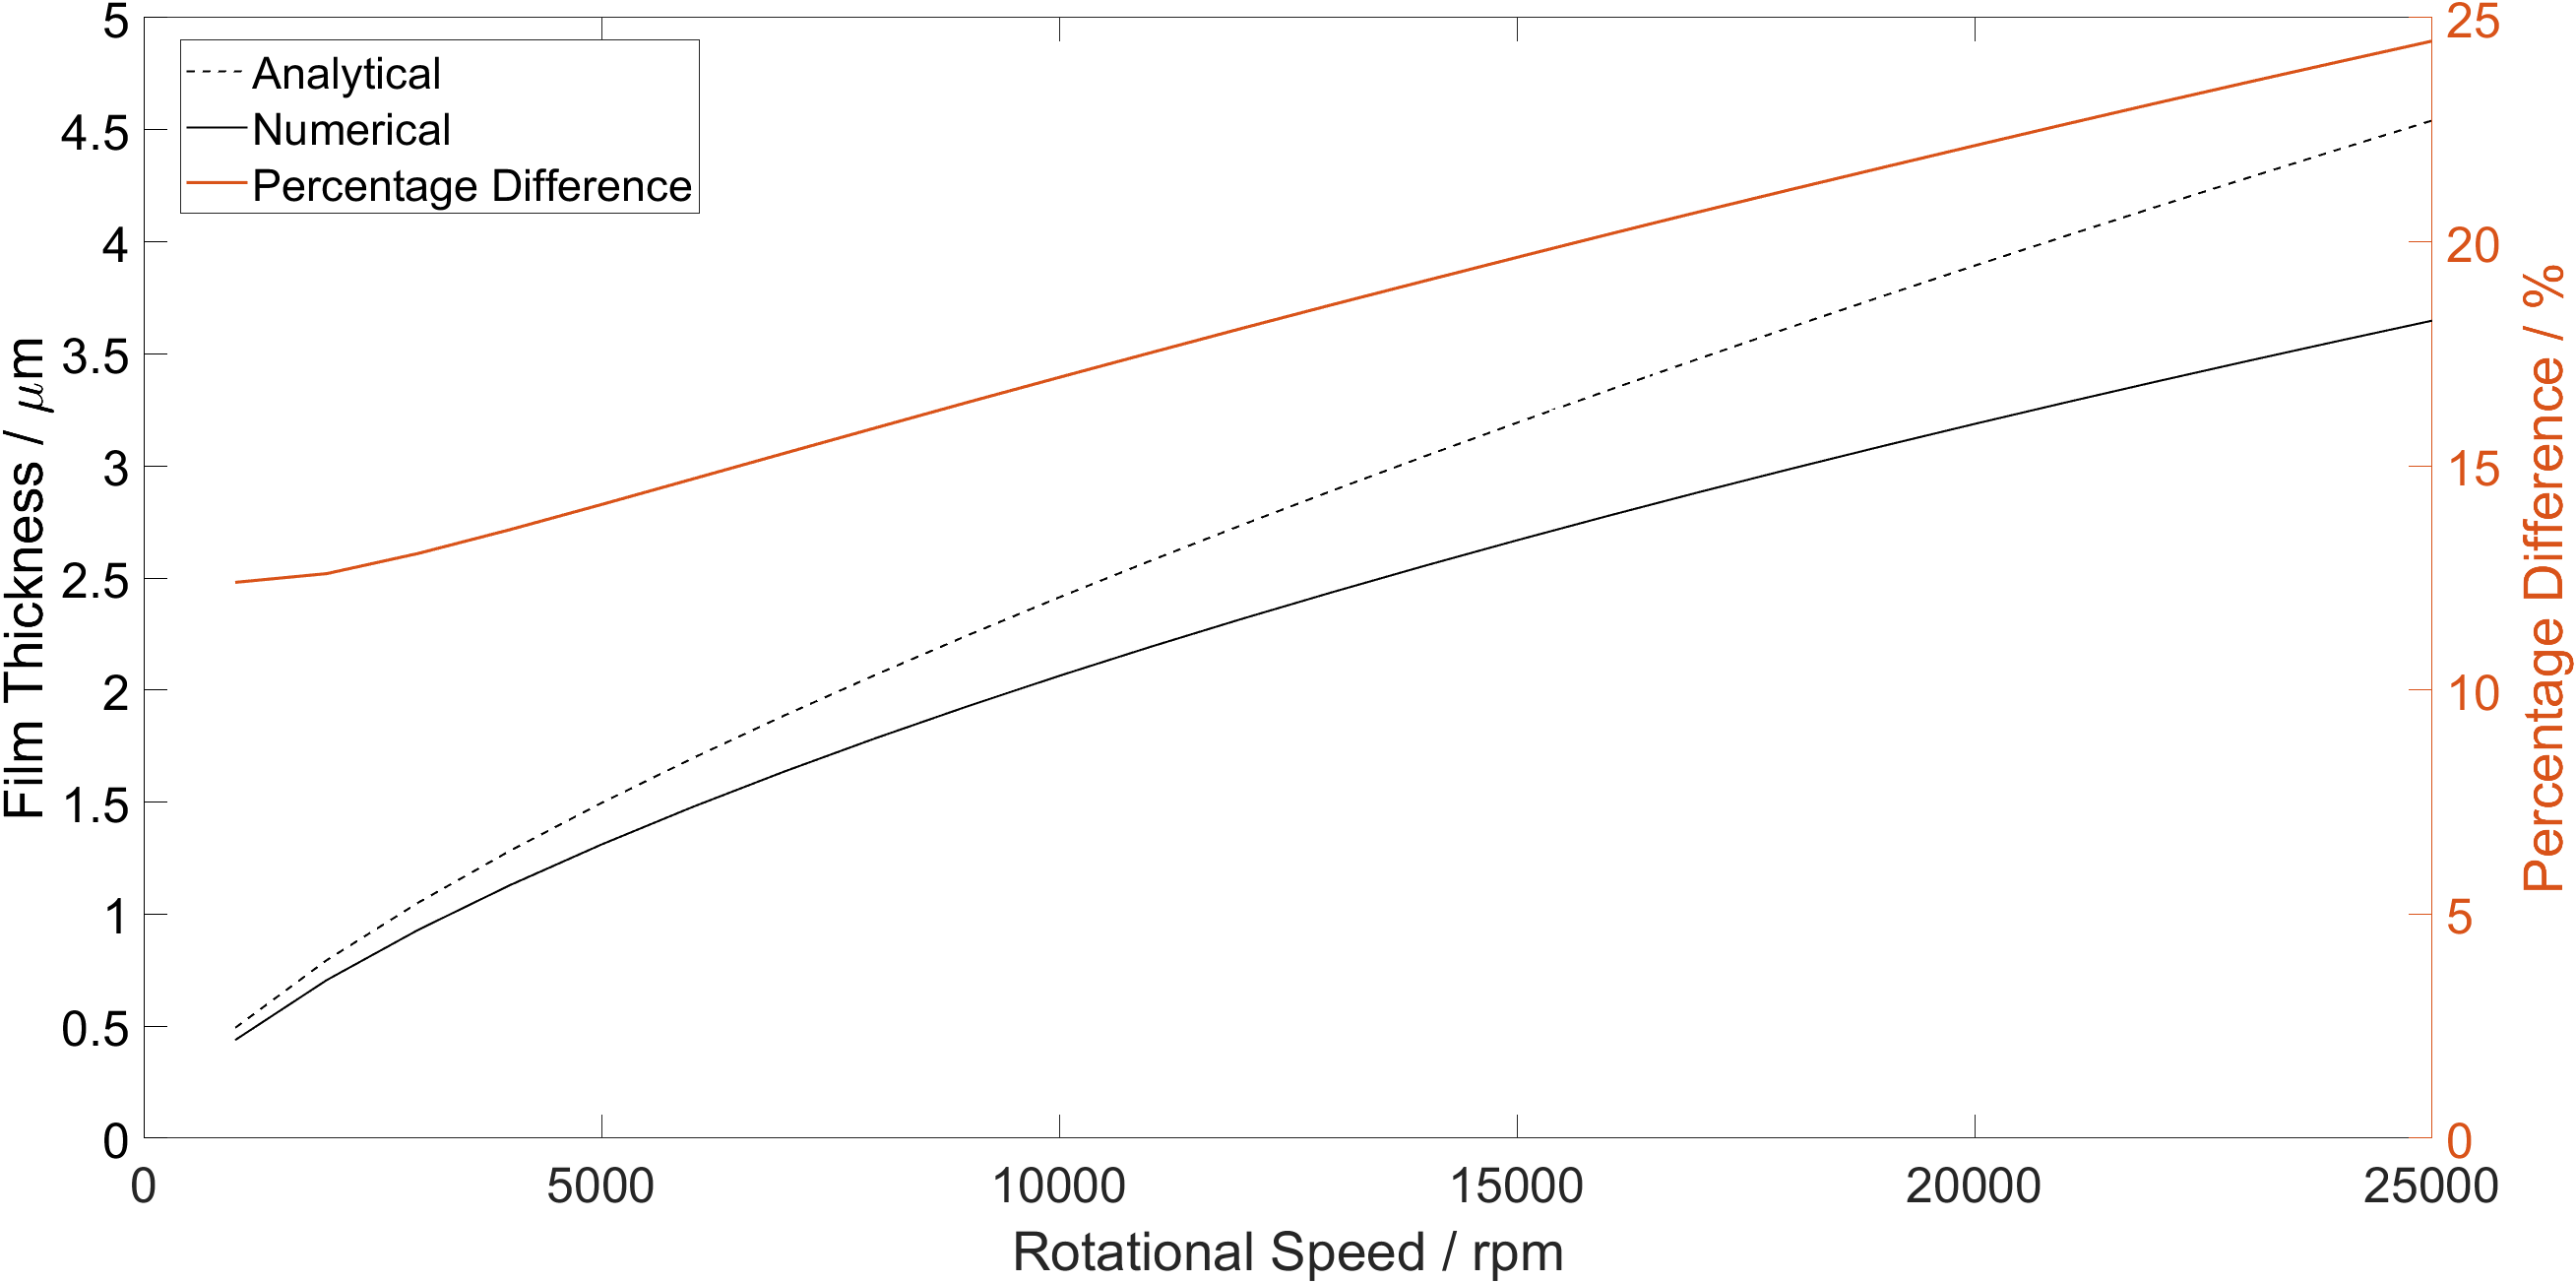
\includegraphics[width=140mm]{EHL_NumericalvsAnalytical_25000.png}
	\caption{Central film thickness - EHL vs analytical.}
	\label{EHL_NumericalvsAnalytical_25000}
\end{figure} 

It is shown that as rotational speed and hence entrainment velocity increase, the film thickness prediction of the numerical and analytical calculations diverge. At 0~-~25~000~$rpm$, entrainment velocities of 38~$m/s$ leads to a 24.5\% difference between the methods, with the analytical equation overestimating the film thickness.

The implementation of ANNs within tribology is one way to overcome the computational expense of the full numerical solution and this limited validity of the analytical approach. Overcoming the above stated discrepancy is not the only advantage of a numerical EHL informed ANN. Since an ANN can be trained using a wide range of input data, the effects of other tribological phenomena such as starvation and thermal effects can be considered. Furthermore, the training of such ANNs is not bound to only numerical inputs; the results of experimental testing could be used to generate an experimentally validated ANN.

\section{ANN Fundamentals}

An Artifical Neural Network (ANN) is a computational model that is inspired by the biological neural networks present in the natural brain \cite{Sarkar2017}. ANNs are a subset of machine learning (ML) that can be trained using supervised, unsupervised, or reinforcement learning techniques. In supervised learning, ANNs are particularly useful for regression tasks, where they can model complex non-linear relationships between inputs and outputs. ANNs compare their outputs with target values during training and, due to their structure, can adapted for a wide range of applications. The goal of this training is to minimize the error, and to improve the ability of the network to generalize and make accurate predictions for new, unseen data.

ANNs consist of a set of interconnected processing elements known as neurons. These are represented computationally as nodes, and the terms are often used interchangeably. These elements have the ability to adapt to input data for the purpose of solving complex non-linear functions. The neurons are organized into three main layers, shown in Figure \ref{ANN schematic}: Input layer; Hidden layer(s) and Output layer. The adaptation is performed using weighted connections that link each neuron layer. These weightings are adjusted during the learning process, and determine the strength of the connections between neurons.

\begin{figure}
	\centering  
	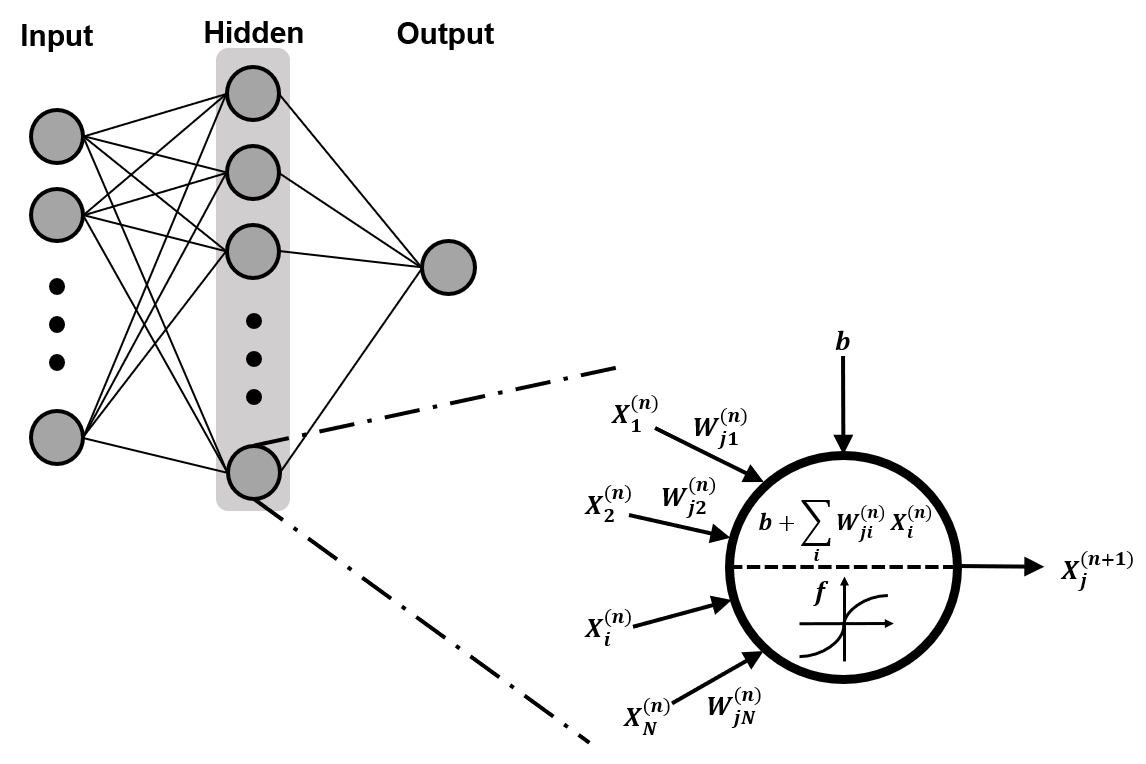
\includegraphics[width=150mm]{ANN_schematic.png}
	\caption{ANN schematic}
	\label{ANN schematic}
\end{figure} 

The following section provides descriptions of the common terms that will be referenced throughout this chapter.

\subsection{Network Architecture}
\begin{itemize}
	\item \textbf{Input layer}: Input data is assigned to input nodes in the first layer of the network. In the case of the film thickness estimation, nine input variables and hence nine nodes are required.
	\item \textbf{Hidden layer(s)}: These layers are located between the input and output layer. There can be multiple hidden layers, each consisting of multiple nodes. Single layer networks are able to solve linear problems, whereas multi-layer networks enable the resolution of non-linear problems \cite{Bell2014}.
	\item \textbf{Output layer}: The output layer contains the final results. In the case of the film thickness estimation, this is simply one node that corresponds to the central film thickness.
\end{itemize}

The type of ANN used in this study is called a multi layer feedforward backpropogation neural network. Forward propogation through the network is used to make prediction, then backpropogation is performed to calculate prediction error and modify the network to minimize this. This process is repeated until the desired prediction accuracy is achieved.

\subsection{Forward Propogation}

Input data propagates through the neural network in the following manner:
\begin{enumerate}
	\item \textbf{Weights}: The input data to the nodes is multiplied by corresponding weights, and a bias term is added (see Figure \ref{ANN schematic}). The general equation for ANNs is:
	
	\begin{equation}\label{Generalized ANN1}
		z = f(b+\sum_i W_{j i}^{(n)} X_i^{(n)})
	\end{equation}
	
	where $z$ represents the activated output of the neuron. $W_{j i}$ is the weight connecting the $i$-th neuron of the previous layer to the $j$-th neuron of the current layer in the $n$-th layer. $X_i^{(n)}$ is the input value to the neuron from the $i$-th neuron in the previous layer. The bias is represented by $b$, and $f$ represents the activation function applied to the weighted sum.
	
	\item \textbf{Activation function}: The weighted sum ($b+\sum_i W_{j i}^{(n)} X_i^{(n)}$) is passed through an activation function, $z$, which introduces non-linearity to the system to enable the learning of complex patterns.
	
	\item \textbf{Bias}: The bias term, $b$, is able to shift the activation function's output. It ensures that a neuron can still activate even in the case where all input values are zero.
	
	\item \textbf{Output generation}: Data is propagated through the system until it reaches the final prediction at the output layer.
\end{enumerate}

\subsection{Backpropagation}

The learning process of an ANN is achieved by adjusting the weights in the network. This is done using a process called backpropagation \cite{Bishop2006}.
\begin{enumerate}
	\item \textbf{Loss function}: During training, the target output of the ANN is known. The predicted output of the ANN is therefore measured against this using a loss function. In the case of ANNs used for regression, mean squared error (MSE) is used.
	\item \textbf{Backpropogation}: This error is backpropogated through the system to determine the contribution of each weight to that error.
	\item \textbf{Optimization}: Optimization algorithms, such as Levenberg-Marquardt \cite{Levenberg1944} \cite{Marquardt1963} \cite{Wilamowski2010}, are used to update the weights and biases to reduce the loss.
	\item \textbf{Epochs}: The above process repeats over multiple cycles, known as epochs. This is performed until the desired MSE is achieved.
\end{enumerate}

For a comprehensive overview of machine learning fundamentals, the reader is referred to CITE. Their application to tribological work is also comprehensively covered by Marian \cite{Marian2021}.

\section{Methodology}

This section details the following methodology:

\begin{enumerate}
	\item Generating training data for the ANN using the numerical EHL method, and constraining this input data to a range valid for machine element contacts.
	\item Evaluating the best ANN structure for the central film thickness estimation.
	\item Testing the ANN using by calculating bearing film thickness explicitly based on kinematic condition obtained from a dynamic bearing model.
	\item Embedding the ANN within a FMBD model to calculate and implicitly consider the film thickness within the bearing at each time step of the simulation.
	
\end{enumerate}

The workflow describing the EHL data generation, variable constraints, training methodology and structure evaluation is presented in Figure \ref{ANN flowchart}. This workflow resulted in a structurally optimised trained ANN that could be used for the explicit and implicit modelling tests.

\begin{figure}  
	\centering
	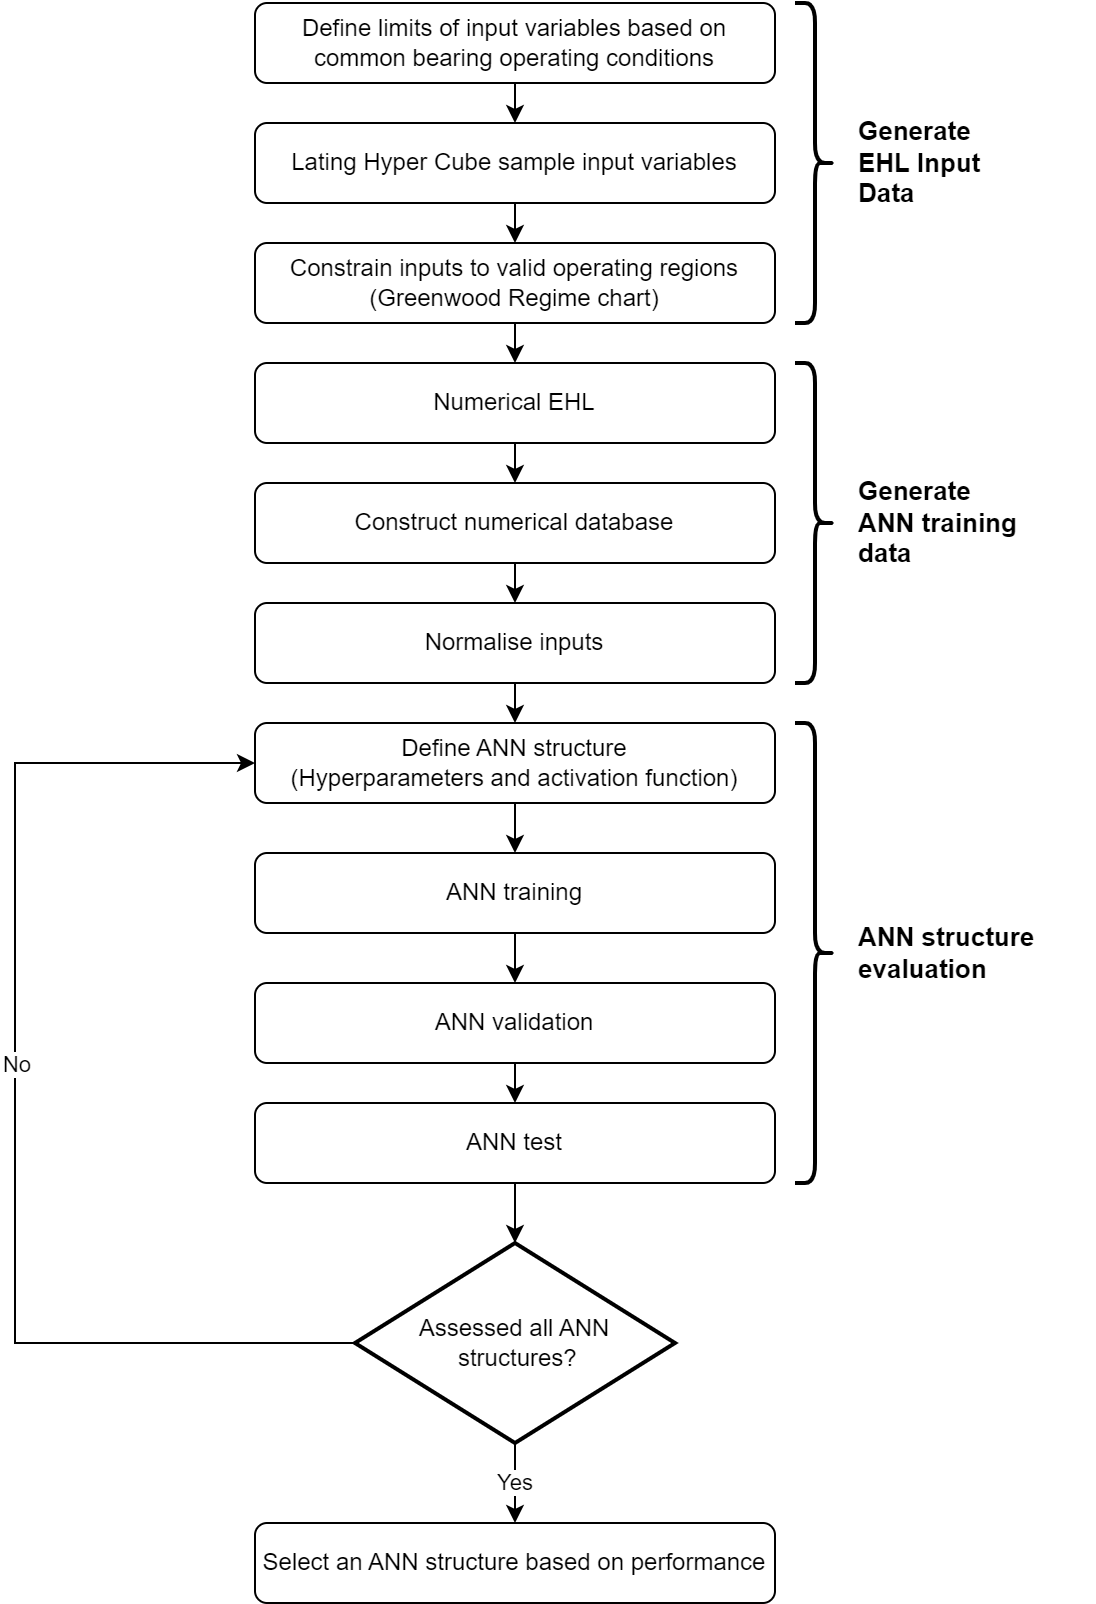
\includegraphics[width=105mm]{ANN_structure_flowchart.png}
	\caption{ANN data flow, models and training flowchart}
	\label{ANN flowchart}
\end{figure} 

\subsection{EHL Input Data Generation}

Training an ANN requires an often comprehensive data set. For this study, the training data was generated using the numerical EHL model presented in \ref{1D EHL Model}. This approach was selected due to the large size of the dataset required for training, and the relatively low resource-intensive nature to generate this. It is important to note that the training data could also be obtained from experimental work, which would further enhance the applicability of this approach for future studies.

\subsubsection{Sampling Input Variables}

Due to the large design space covered by the high number and range of input parameters, a robust sampling technique must be chosen to create the training data set. In traditional random sampling, each of the parameters is randomly sampled within its defined range. This may lead to insufficient coverage of the parameter space and simple bias, as it lacks a systematic approach to ensure even distribution \cite{Preece2016}.

The Latin Hypercube Sampling (LHS) method was utilised by Marian et al. \cite{Marian2022}, and was chosen for this study. It is a statistical method used to efficiently sample a high-dimensional parameter space, such as that required for the central film thickness calculation. LHS is derived from Latin Hypercube Design (LHD), where each parameter’s range is divided into equal intervals along each dimension. Each interval is then randomly assigned to a unique position within its corresponding dimension. The process results in a matrix, where each row represents a combination of parameter values. Contrary to the random sampling method, LHS ensures that each interval is sampled exactly once per dimension, preventing clustering and improving representation across the space \cite{Preece2016}. This ensures lower computational effort required for ANN training, despite the high number of input variables and value ranges.

The LHD is a $n_{\mathrm{s}} \times n_{\mathrm{f}}$ matrix, where $n_s$ and $n_f$ represent the number of simulations the number of factors respectively. LHS enhances LHD by introducing a randomization component. The randomly selected samples within each interval undergo permutation, ensuring that samples are not biased by the order of selection.

LHS elements are generated by subtracting a random number between zero and one $Z_{\mathrm{r}}\in[0,1]$ from each LHD element $x_{i j, \mathrm{LHD}}$. This is then divided by the number of test points \cite{Siebertz2010}:

\begin{equation}\label{LHS}
	x_{i j, \mathrm{LHS}}=\frac{x_{i j, \mathrm{LHD}}-Z_{\mathrm{r}}}{n_{\mathrm{s}}}
\end{equation}

This equation rescales the LHD values to a range between 0 and 1. By subtracting a random number between 0 and 1 and dividing by the total number of sample points, the resulting Latin hypercube samples are spread evenly across the interval (0,1) for each parameter. This is important, because it allows the Latin hypercube samples to be easily transformed to any desired range or distribution. This transformation to the design space is done using the limits of the tribological parameters in Table \ref{Sensitivity study of ANN structure}.

The quality of the test field (freedom of correlation and uniform distribution) can be assessed based on the distances between data points \cite{Johnson1990}. The MaxiMin criterion in the MATLAB\textregistered\ Statistics and Machine Learning toolbox was used to optimise the LHS. This maximises the the minimum distance between individual test points such that the LHS test field is uniformly distributed:

\begin{equation}\label{maximin}
	\operatorname{MaxiMin}=\left[\sum_{1 \leq i<j \leq n_1} d\left(x_i, x_j\right)^{-\xi}\right]^{-\frac{1}{\xi}}
\end{equation}

where $d$ represents all distances in the test field, and subscripts $i$ and $j$ are indexes for the parameter and sample point respectively. $\xi$ represents the application dependant factor which determines the degree of importance assigned to the distances \cite{Siebertz2010}.

\subsubsection{Constraining the Input Data Bounds}

The performance of ANNs is heavily reliant upon the quality of the data set provided for training. To construct a training database, Marian et al. \cite{Marian2022} utilised a Finite Element Method (FEM) solver for film thickness calculations. The database covered a very large range of lubricant and material properties for relatively low entrainment speed conditions (< 0.4~$m/s$ for the 2D line contact studies). Contact conditions for some combinations of these input parameters exceed realistic conditions within common machine elements, including bearings. To further improve upon this methodology, the input data range required constraining.

The Greenwood Regime chart \cite{Johnson1970} was used for this purpose. The regions of the chart, as shown in Figure \ref{Greenwood informed training data vs Marian et al.}, are:

\begin{itemize}
	\item Isoviscous Rigid (IR)
	\item Isoviscous Elastic (IE)
	\item Piezoviscous Rigid (PR)
	\item Piezoviscous Elastic (PE)
\end{itemize}

The bounds indicate the transition between the lubrication regimes, which are classified based on material, rheological and geometric properties. To find which regime a contact is operating within, the dimensionless elasticity ($G_e$) and viscosity ($G_v$) parameters can be calculated:

\begin{equation}\label{G_e}
	G_e=\left(\frac{\alpha^2 W_i^3}{\eta_0 u R_r^2}\right)^{\frac{1}{2}}
\end{equation}

\begin{equation}\label{G_v}
	G_v=\left(\frac{W_i^2}{\eta_0 u E_r R_r}\right)^{\frac{1}{2}}
\end{equation}

The PE region signifies and EHL contact, where pressure are high enough to elastically deform the material and increase the viscosity of the lubricant. The IR region relates to the hydrodynamic regime of lubrication, where the contact load does not deform the surface and viscosity remains constant. Since these investigations are focussed on improving the EHL film thickness estimation, the training data set was required to fall within the PE region of the Greenwood plot. 

The initial range of each parameter is shown in Table \ref{Range of ANN film thickness calculation parameters}. A training data set was then generated using these limits. The input data was then constrained further to ensure Hertzian pressures, $P$, were between 300~$MPa$ and 3.5~$GPa$, as well as redistributing any points that fell outside of the PE and PR regions. A flowchart to explain the process of constraining the input variables is shown in Figure \ref{EHL_Greenwood_Constraints_Flowchart}.

\begin{figure}
	\centering  
	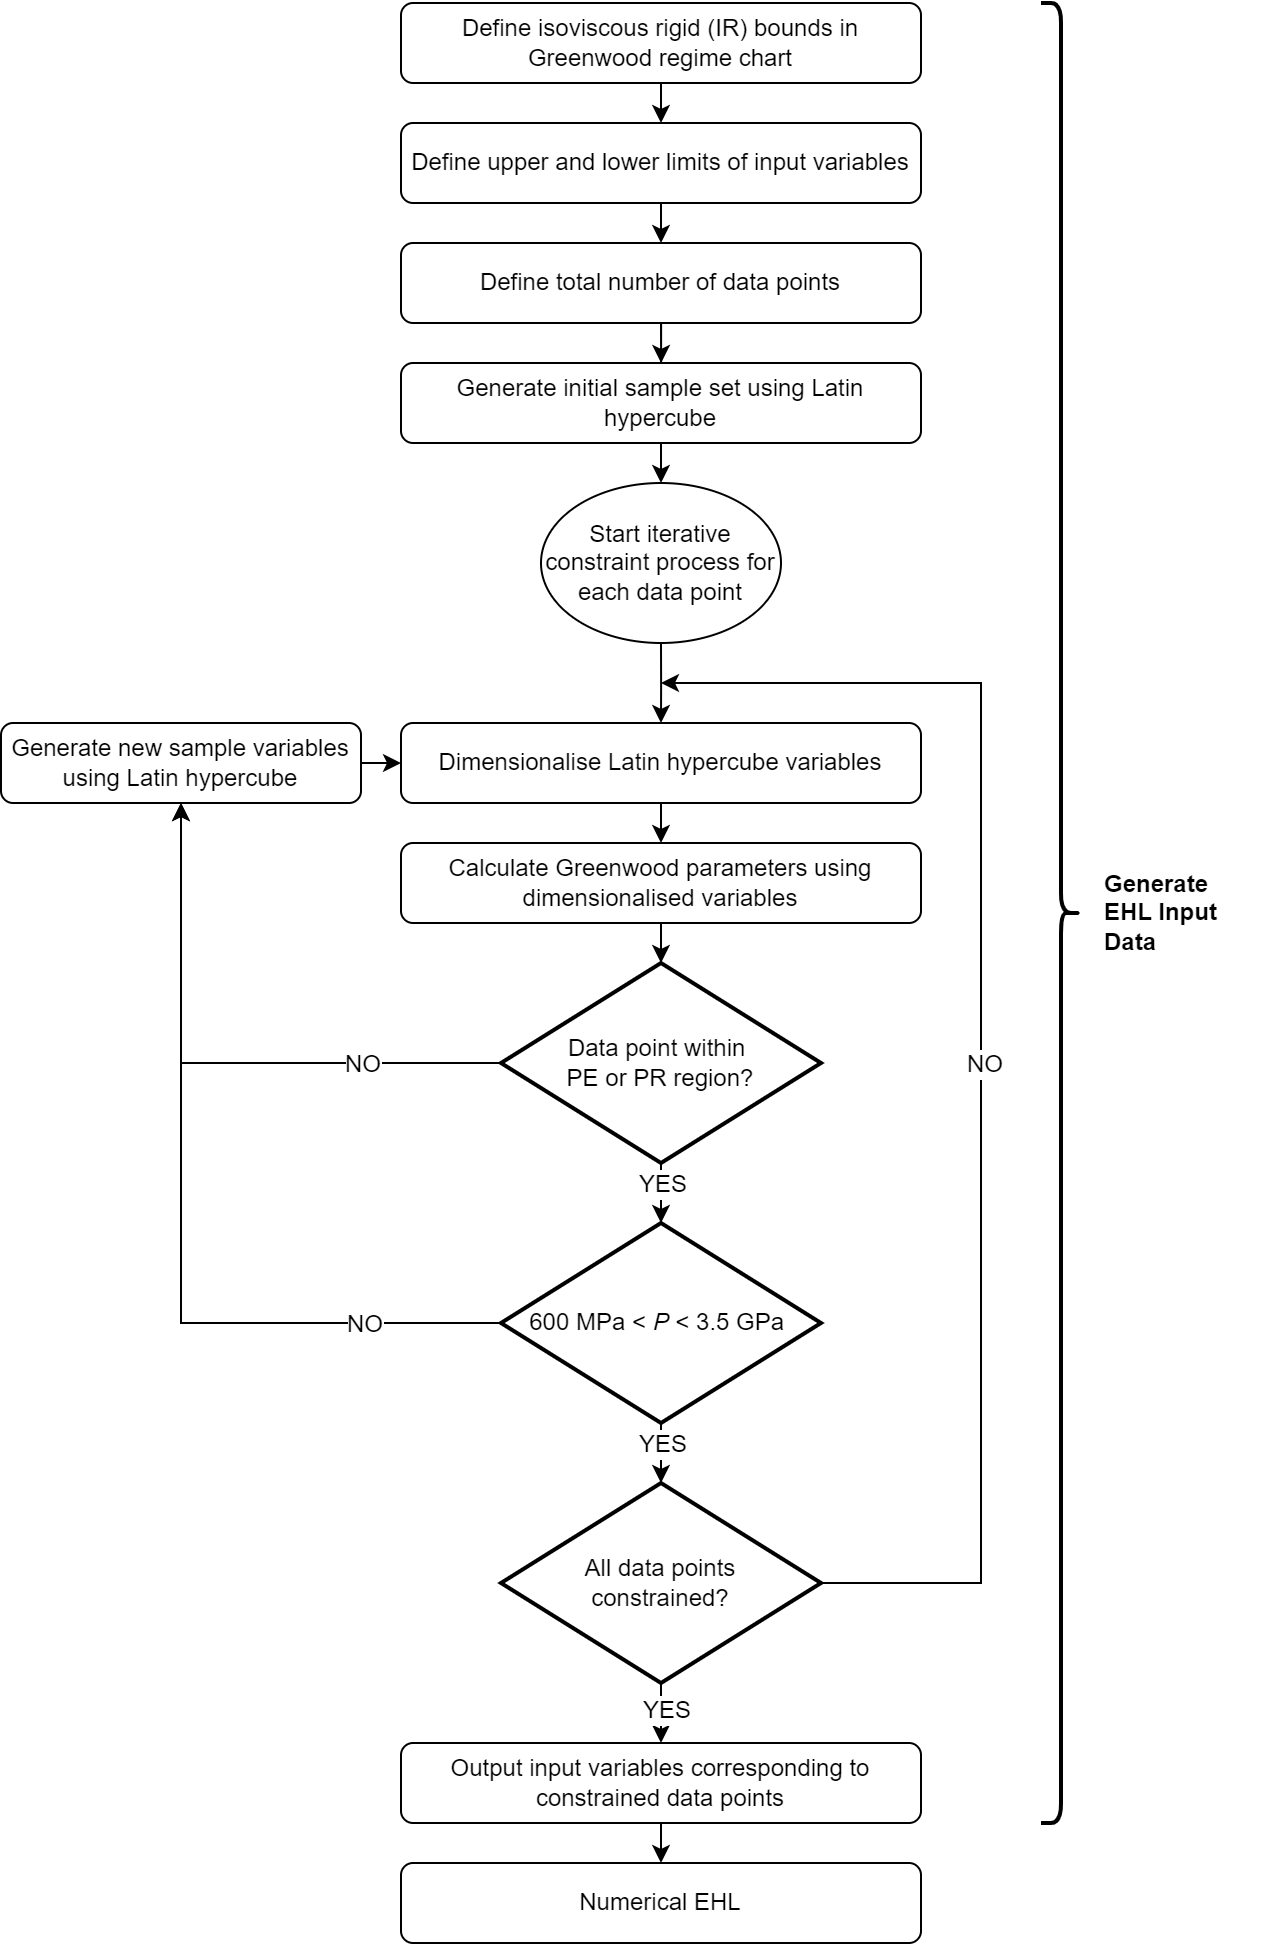
\includegraphics[width=130mm]{EHL_Greenwood_Constraints_Flowchart.png}
	\caption{Workflow to constrain training input data using Greenwood regimes}
	\label{EHL_Greenwood_Constraints_Flowchart}
\end{figure} 

\begin{figure}
	\centering  
	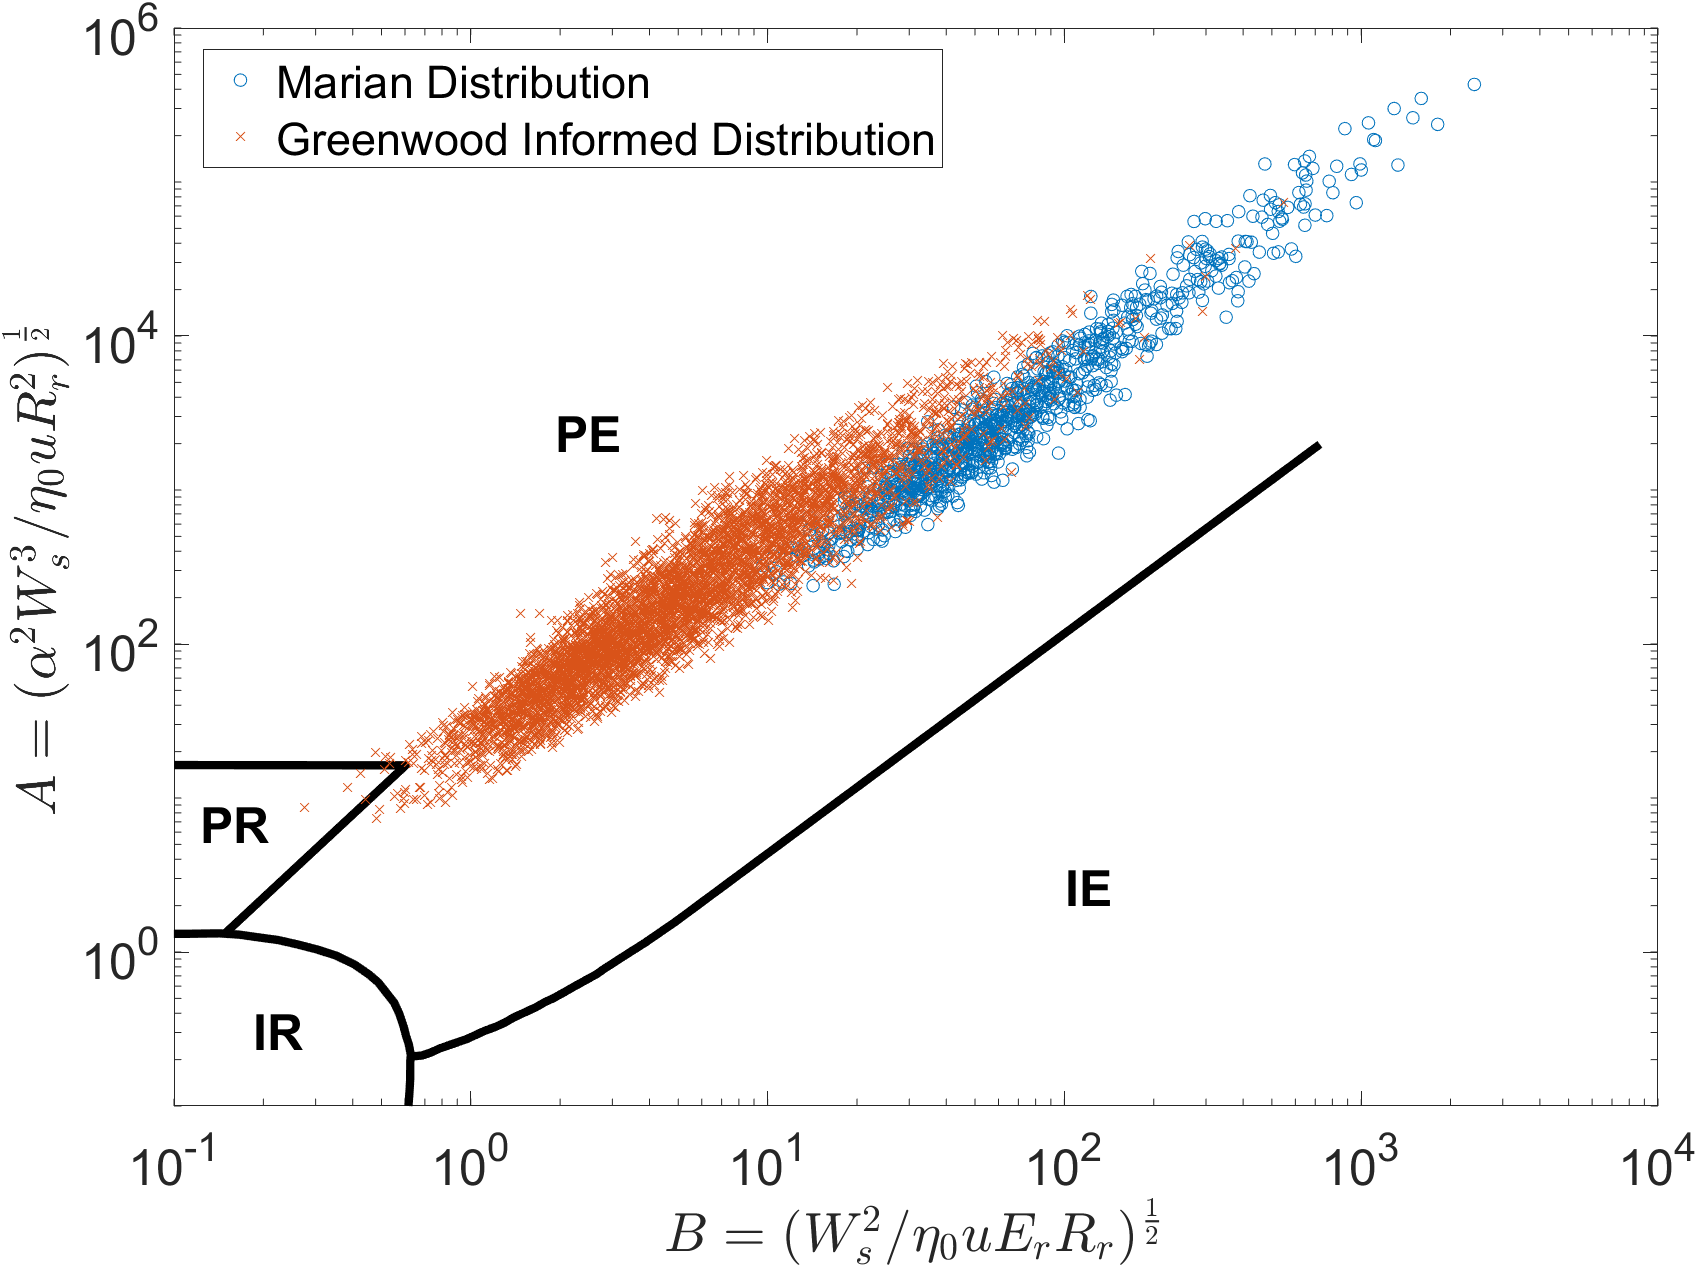
\includegraphics[width=150mm]{ANN_Explicit_MarianvsGreenwood.png}
	\caption[Greenwood informed training data vs Marian et al.]{Greenwood informed training data vs Marian et al. \cite{Marian2022}.}
	\label{Greenwood informed training data vs Marian et al.}
\end{figure} 

\begin{table*}
	%\captionsetup{justification=centering}
	\caption{Range of ANN film thickness calculation parameters}
	\label{Range of ANN film thickness calculation parameters}
	\centering
	\renewcommand{\arraystretch}{1.5}%
	\begin{tabular}{|P{0.4\textwidth}|P{0.15\textwidth}|P{0.15\textwidth}|P{0.15\textwidth}|}
		\hline
		\textbf{Parameter} & \textbf{Unit} & \textbf{Minimum} & \textbf{Maximum} \\ [0.5ex]
		\hline
		Load & $N$ & 150 & 5000 \\ [0.5ex]
		\hline
		Entraining Velocity & $m/s$ & 0.6 & 30 \\ [0.5ex]
		\hline
		Reduced Radius & $m$ & 0.0001 & 0.02 \\ [0.5ex]
		\hline
		Reduced Elastic Modulus & $GPa$ & 200 & 250 \\ [0.5ex]
		\hline
		Pressure-Viscosity Coefficient & ${GPa}^{-1}$ & 10 & 30 \\ [0.5ex]
		\hline
		Reference Viscosity & $Pa.s$ & 0.0005 & 0.1 \\ [0.5ex]
		\hline
		Maximum Density & ${kg}/{m}^3$ & 7750 & 8050 \\ [0.5ex]
		\hline
		Poisson's Ratio & $-$ & 0.3 & 0.35 \\ [0.5ex]
		\hline
		Contact Length & $m$ & 0.001 & 0.050 \\ [0.5ex]
		\hline
		
	\end{tabular}
\end{table*}

A comparison of an the unconstrained and constrained input variables used for the training data is shown in Figure \ref{Training_Unconstrained_GreenwoodRegime}. It is shown that for the same number of data points (5~000), the data cloud is concentrated over a smaller region of the chart. This improved the point density in regions of interest, increasing the likelihood that the training data more closely matches the test data.

\begin{figure}
	\centering  
	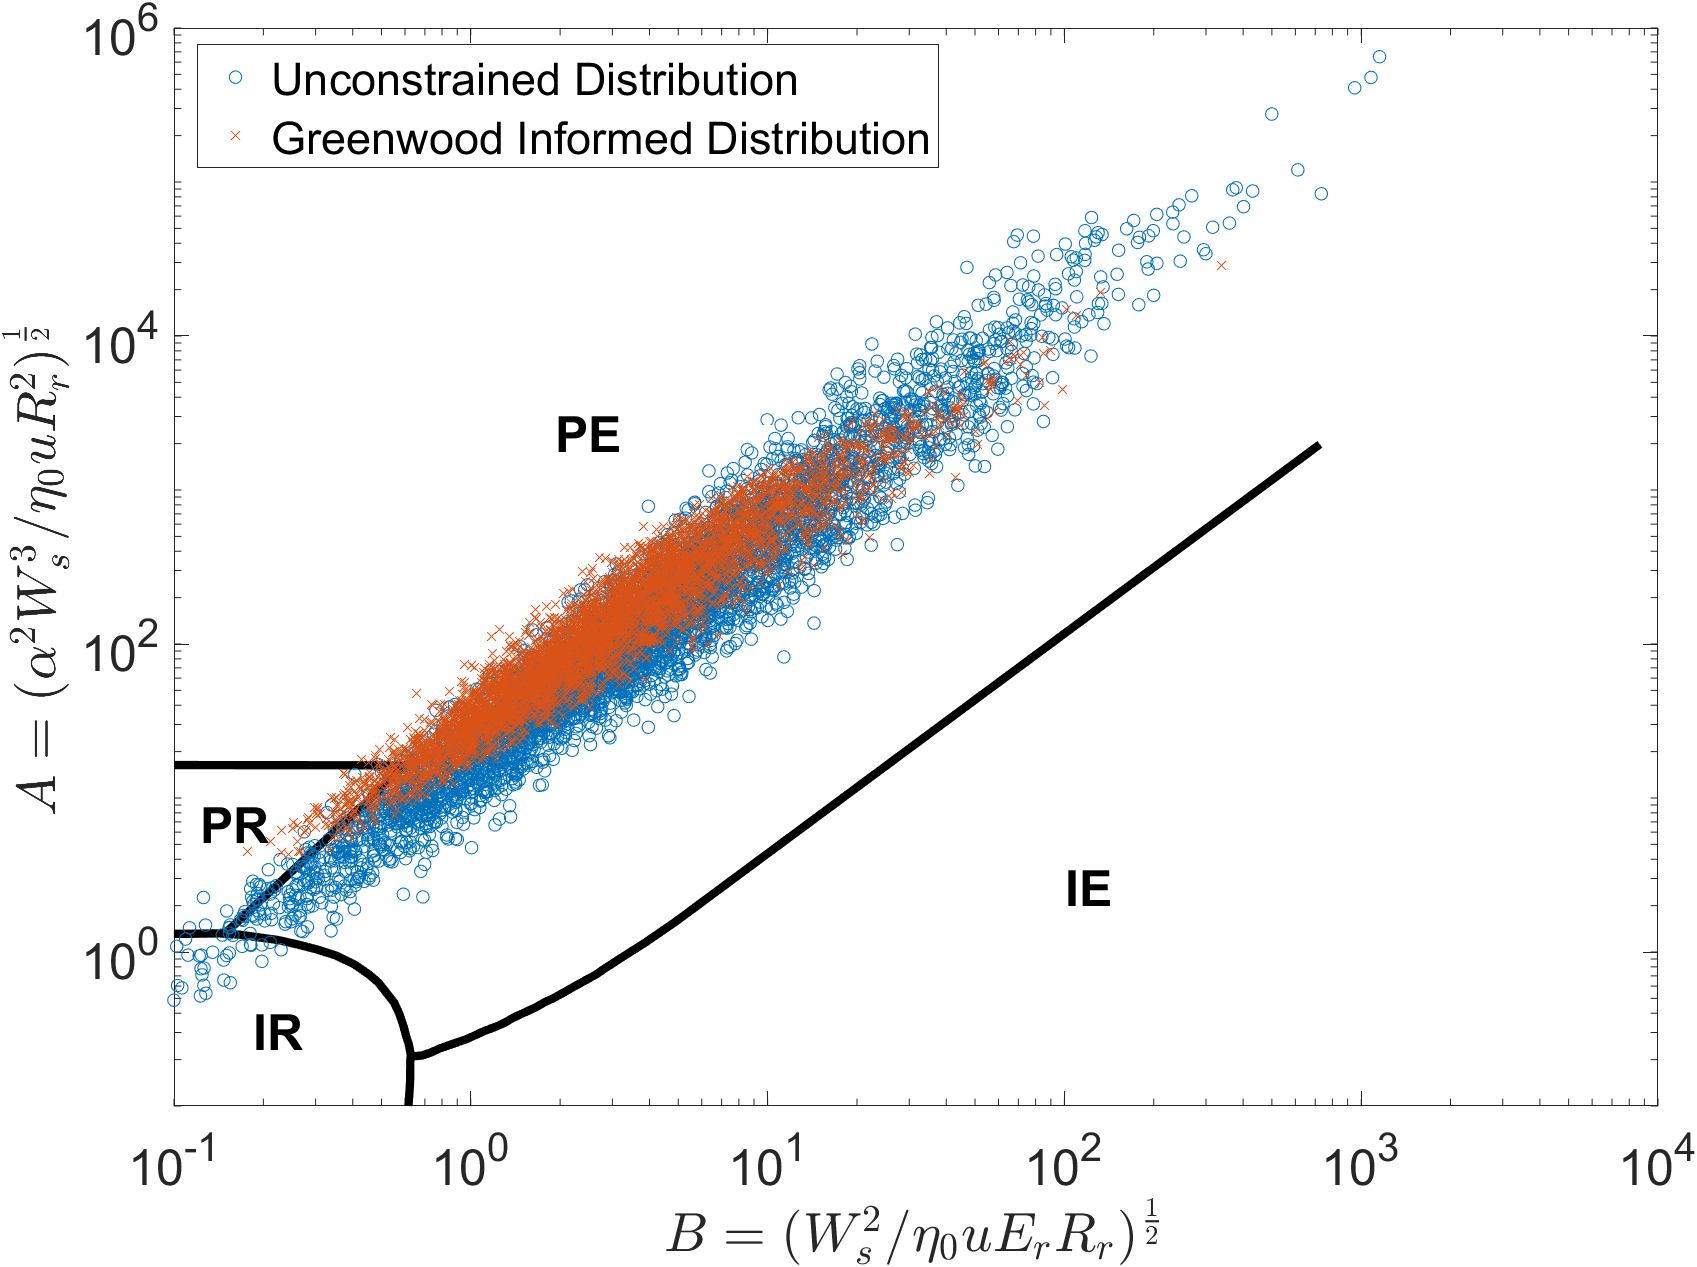
\includegraphics[width=150mm]{Training_Unconstrained_GreenwoodRegime.png}
	\caption{Greenwood informed training data vs unconstrained data.}
	\label{Training_Unconstrained_GreenwoodRegime}
\end{figure} 

\subsubsection{Constructing the Numerical Database}

The 1D EHL model presented in Section \ref{1D EHL Model} was used to generate the numerical database for training the ANN. The variables corresponding to each constrained data point in Figure \ref{Training_Unconstrained_GreenwoodRegime} were used as inputs to the calculation. The target output of central film thickness was calculated.

\subsection{ANN Structure Evaluation}

The general structure of the ANN is described in the following format, as per \cite{Zhang2002}:

\begin{equation}
	N_{i n}-\left[N_{h 1}-N_{h 2}-N_{h 3}\right]_t-N_{\text {out }}
\end{equation}

The number of neurons in each layer is denoted by $N$, with the input and output layers indicated by the subscripts $in$ and $out$, respectively. Subscripts $h1$, $h2$, and $h3$ denote the hidden layers, with $t$ being the total number of hidden layers. A graphic representation of the structure used for the film thickness estimations is show in Figure \ref{ANN structure}. As the structural complexity of ANNs increases, the training time increases due to the greater number of neurons and layers. Implementations of ANN in the field of tribology, specifically film thickness predictions, are typically limited to between one and three hidden layers \cite{Marian2021}.

\begin{figure}
	\centering  
	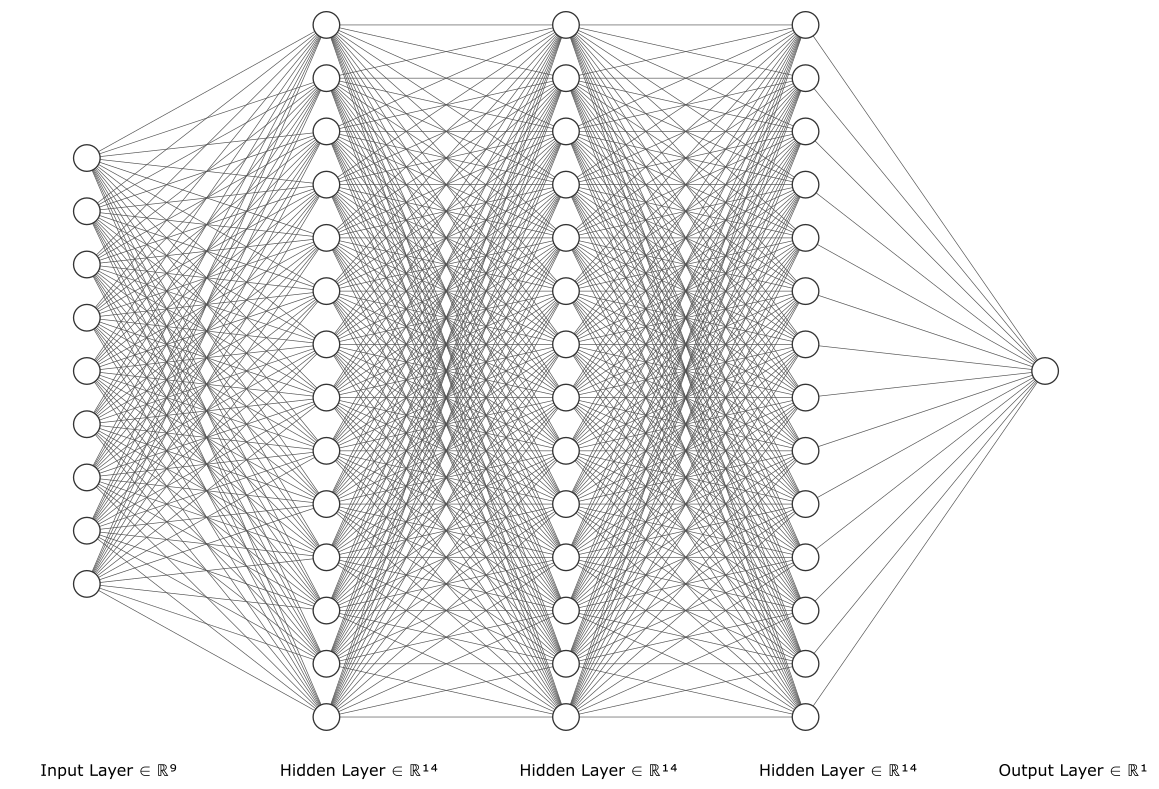
\includegraphics[width=150mm]{ANN_Structure.png}
	\caption{ANN structure to predict EHL central film thickness ($9-[14-14-14]_3-1$)}
	\label{ANN structure}
\end{figure} 

The structure of an ANN affects both its training time and prediction accuracy. To evaluate the performance of different ANN structures, and hence select an appropriate structure for this application, a sensitivity study was performed.

The study comprised of over 500 different ANN structures. The input data range remained constant across all structures, while the variables listed in Table \ref{Sensitivity study of ANN structure} were adjusted. The number of hidden layers was varied between one and four, and the number of neurons between 10 and 20. Three activation functions: Hyperbolic tangent, Logistic sigmoid and Rectilinear were evaluated.

Selection of the final structure for suitability analysis was based on total training time, coefficient of determination ($R^2$), and the potential for the ANN to overfit. Overfitting is the phenomenon whereby an ANN becomes too specialised at learning the training data, and as a result performs poorly with new, unseen data. This occurs when the network extensively adjusts its internal parameters to fit noise or outliers in the training set \cite{Ying2019}.

\begin{table*}
	%\captionsetup{justification=centering}
	\caption{Sensitivity study of ANN structure}
	\label{Sensitivity study of ANN structure}
	\centering
	\renewcommand{\arraystretch}{1.5}%
	\begin{tabular}{|P{0.4\textwidth}|P{0.4\textwidth}|}
		\hline
		\textbf{Variable} & \textbf{Value} \\ [0.5ex]
		\hline
		Number of training data points & 600 - 1500 \\ [0.5ex]
		\hline
		Number of hidden layers, t & 1 - 4 \\ [0.5ex]
		\hline
		Number of neurons, N & 10 - 20 \\ [0.5ex]
	    \hline
		Activation function type & Hyperbolic tangent, Logistic sigmoid, Rectilinear \\ [0.5ex]
		\hline
	\end{tabular}
\end{table*}

\subsubsection{Data Normalization}

Normalization of the input and target parameters is first performed using the min-max normalisation function:

\begin{equation}
	\tilde{x}=\frac{x-x_{\min }}{x_{\max }-x_{\min }}(u-l)+u
\end{equation}

where $u$, and $l$ represent the upper and lower normalized unit values of 1 and -1 respectively. The dimensional target input value is denoted by $x$, and the final normalised input or output parameter of the ANN is denoted by $\tilde{x}$. In order to dimensionalise the output layer, $x_{\max }, x_{\min }$ must be stored as a variable.

\subsubsection{Training, Validation and Test Datasets}

The dataset is divided into three sets: the training set, the validation set, and the test set, each containing 70~$\%$, 15~$\%$ and 15~$\%$ of the training data respectively:

\begin{enumerate}
	\item \textbf{Training Set}: The training set is the portion of the dataset used to train the ANN, containing the input data and the corresponding output data. As aforementioned, the ANN adjusts the internal parameters based on this data to learn the underlying patterns.
	\item \textbf{Validation Set}: The validation set is used to tune the performance of the ANN during the training process. It is an independent dataset that the network has not seen before, allowing for the evaluation of its generalization capabilities. The network's performance on the validation set is monitored during training to make decisions on adjusting hyperparameters (number of hidden layers, neurons per hidden layer, activation functions), or stopping the training process to prevent overfitting.
	\item \textbf{Test Set}: The test set is a completely independent dataset that is not used during training or validation. It is used to assess the final performance and generalization ability of the trained ANN. By evaluating the network on unseen data, the test set provides an unbiased estimate of the model's performance in actual use.
\end{enumerate}

For this sensitivity study, the size of the training data set was varied (600, 1000, 2000 and 5000) to observe the its effect on the quality of the predictions. A limit of 1000 epochs was also implemented, restricting the ANN to 1000 full iterations through the entire training set. This was found to be sufficient to improve accuracy while preventing overfitting.

\subsubsection{Evaluating the Network Performance}

During backpropagation of the ANN, the Mean Squared Error (MSE) was used to evaluate the network's performance:

\begin{equation}\label{MSE}
	M S E=\frac{1}{N} \sum_{i=1}^N\left(t_i-y_i\right)^2
\end{equation}

where $t_i$ and $y_i$ are the target and predicted value respectively. The total number of training points being trained, validated or tested is denoted by $N$. 

To assess the goodness of fit of the ANN, the statistical metric $R^2$, known as the coefficient of determination, was used. This measures the proportion of variance in the dependant variable (film thickness) that is predictable from the input variables (Table \ref{Range of ANN film thickness calculation parameters}) in the model. This value ranges from 0 to 1, with a higher value indicating the best fit of the model to the data. This was post-processed after training and is calculated as follows:

\begin{equation}\label{R-squared}
	R^2=1-\frac{\sum_{i=1}^N\left(t_i-y_i\right)^2}{\sum_{i=1}^N\left(y_i-\bar{y}\right)^2}
\end{equation}

 where $\overline{\mathrm{y}}$ is the mean of the target sample. The numerator of the fraction, \( \sum_{i=1}^N(t_i - y_i)^2 \), represents the sum of squared residuals, which quantifies the variation in the target variable that is not explained by the model. The denominator, \( \sum_{i=1}^N(y_i - \bar{y})^2 \), is the total sum of squares, which captures the total variation in the target variable \cite{Marian2022}.

\subsubsection{Activation Functions}

Activation functions are mathematical functions that are applied to the output of each neuron in a layer of the neural network. These introduce non-linearity which allow the network to learn complex input-output relationships. Activation functions help determine the output of a neuron based on the weighted sum of its inputs.

As suggested in \cite{Marian2022}, suitable activation functions for the hidden layers are as follows:

\begin{itemize}
	\item \textbf{Sigmoid (logistic)}: This function transforms the input values into a range between 0 and 1. It has continuously differentiable smooth S-shaped curve and is given by the following formula \cite{Han1995}:
	
	\begin{equation}\label{Logistic sigmoid}
		\log \operatorname{sig}(x)=\frac{1}{1+e^{-x}}
	\end{equation} 
	
	Sigmoid functions are commonly used in the hidden layers of ANNs, however may suffer from the "vanishing gradient" problem where the partial derivative reaches zero \cite{Sharma2020}, leading to slower convergence during training.
	
	\item \textbf{ReLU (Rectified Linear Unit)}: This function is the most commonly used activation function. It outputs the input value directly if it is positive, and zero otherwise. The mathematical definition is:
	
	\begin{equation}\label{ReLU}
		\operatorname{ReLU}= \begin{cases}x, & x \geq 0 \\ 0, & x \leq 0\end{cases}
	\end{equation}
	
	The gradient is 1 when the neuron is activated, and zero when it is deactivated. This function is computationally efficient and addresses the vanishing gradient problem to an extent \cite{Sharma2020}.
	
	\item \textbf{Tanh (Hyperbolic Tangent)}: The hyperbolic tangent or tanh function is defined as:
	
	\begin{equation}\label{Hyperbolic tangent}
		\tanh (x)=\frac{2}{1+e^{-2 x}}-1
	\end{equation}
	
	The formulation and behaviour is very similar to sigmoid. It produces values which range from -1 to 1, having a centred mean around zero. Like sigmoid, this also experiences vanishing gradients.
	
	\item \textbf{Linear}: A simple linear activation was used on the output.
	
\end{itemize}

Early stopping and regularisation was used to prevent statistical overfitting during training \cite{MatlabOverfit}. Early stopping halts the training process before the model reaches the maximum number of epochs. This is done by monitoring the performance (MSE (Equation \ref{MSE})) of the network against the validation set during training. Once the performance reaches a plateau, or begins to degrade, the training is stopped early. Regularisation adds additional constraints to the learning process. It modifies the performance criteria by accounting for the change in mean square of the network weights and biases (Mean Squared Weight (MSW)). This is calculated in Eq. \ref{MSW}: 

\begin{equation}\label{MSW}
	M S W=\frac{1}{N} \sum_{j=1}^N w_j^2
\end{equation}

where $w_j$ is the individual weight value associated with the $j$-th neuron or connection in the network.

By applying an adjustment factor, denoted as $\gamma^{\prime}$, the weights and biases can be reduced during propagation (Eq. \ref{MSE adjusted}), thus mitigating the risk of overfitting and improving the network's generalization capability.

\begin{equation}\label{MSE adjusted}
	M S E_{r e g}=\gamma^{\prime} * M S W+\left(1-\gamma^{\prime}\right) * M S E
\end{equation}

A parameter study was conducted to determine the optimal structure for the ANN. Over 500 different structures were tested using the same input data. This involved varying the hyperparameters: the number of hidden layers varied from one to four, and the number of neurons from ten to twenty. The three aforementioned activation functions were explored in different hidden layer configurations. This included a combination of hyperbolic tangent in the hidden layers, with the final layer utilizing a logistic tangent function. For each configuration, the values of $R^2$ (coefficient of determination) and the training completion time were documented.

\subsubsection{Structure Sensitivity Study}


The training and numerical calculations were performed using a single core on consumer grade hardware, with the following specifications: Intel\textregistered\ Core\textsuperscript{TM} i7-9750H CPU 6 cores @ 2.60GHz, 32GB RAM; GPU: NVDIA GeForce GTX 1650. The wall time for each calculation was recorded, as well as the total training time of each ANN structure.


\subsection{Explicit Bearing Film Thickness Predictions}

The FMBD model used in Chapter \ref{Lubricated FMBD} was used for this study. The shaft was modelled as a rigid body, and loading was purely static in one radial direction to remove the influence of dynamic effects. The shaft was constrained to one rotational and two lateral degrees of freedom. Bearing properties and operating conditions are shown in Table \ref{Roller bearing parameters} and Table \ref{Operating Conditions} respectively.

\begin{table*}
	%\captionsetup{justification=centering}
	\caption{Roller Bearing Parameters}
	\label{Roller bearing parameters}
	\centering
	\renewcommand{\arraystretch}{1.5}%
	\begin{tabular}{|c|c|}
		\hline
		\ \textbf{Parameter} & \textbf{Value} \\ [0.5ex]
		\hline
		Inner race diameter & 31.5 $mm$ \\ [0.5ex]
		\hline
		Roller diameter & 7.5 $mm$ \\ [0.5ex]
		\hline
		Roller length & 15 $mm$ \\ [0.5ex]
		\hline
		Number of rollers & 12 \\ [0.5ex]
		\hline
		Radial interference & 5 $\mu \mathrm{m}$ \\ [0.5ex]
		\hline
		Young's modulus & 218 $GPa$ \\ [0.5ex]
		\hline
		Poisson's ratio & 0.33 \\ [0.5ex]
		\hline
	\end{tabular}
\end{table*}

\begin{table*}
	%\captionsetup{justification=centering}
	\caption{Operating Conditions}
	\label{Operating Conditions}
	\centering
	\renewcommand{\arraystretch}{1.5}%
	\begin{tabular}{|c|c|}
		\hline
		\ \textbf{Parameter} & \textbf{Value} \\ [0.5ex]
		\hline
		Radial force & 2500 $N$ \\ [0.5ex]
		\hline
		Rotational velocity & 10~000$rpm$ \\ [0.5ex]
		\hline
	\end{tabular}
\end{table*}

\begin{figure}
	\centering  
	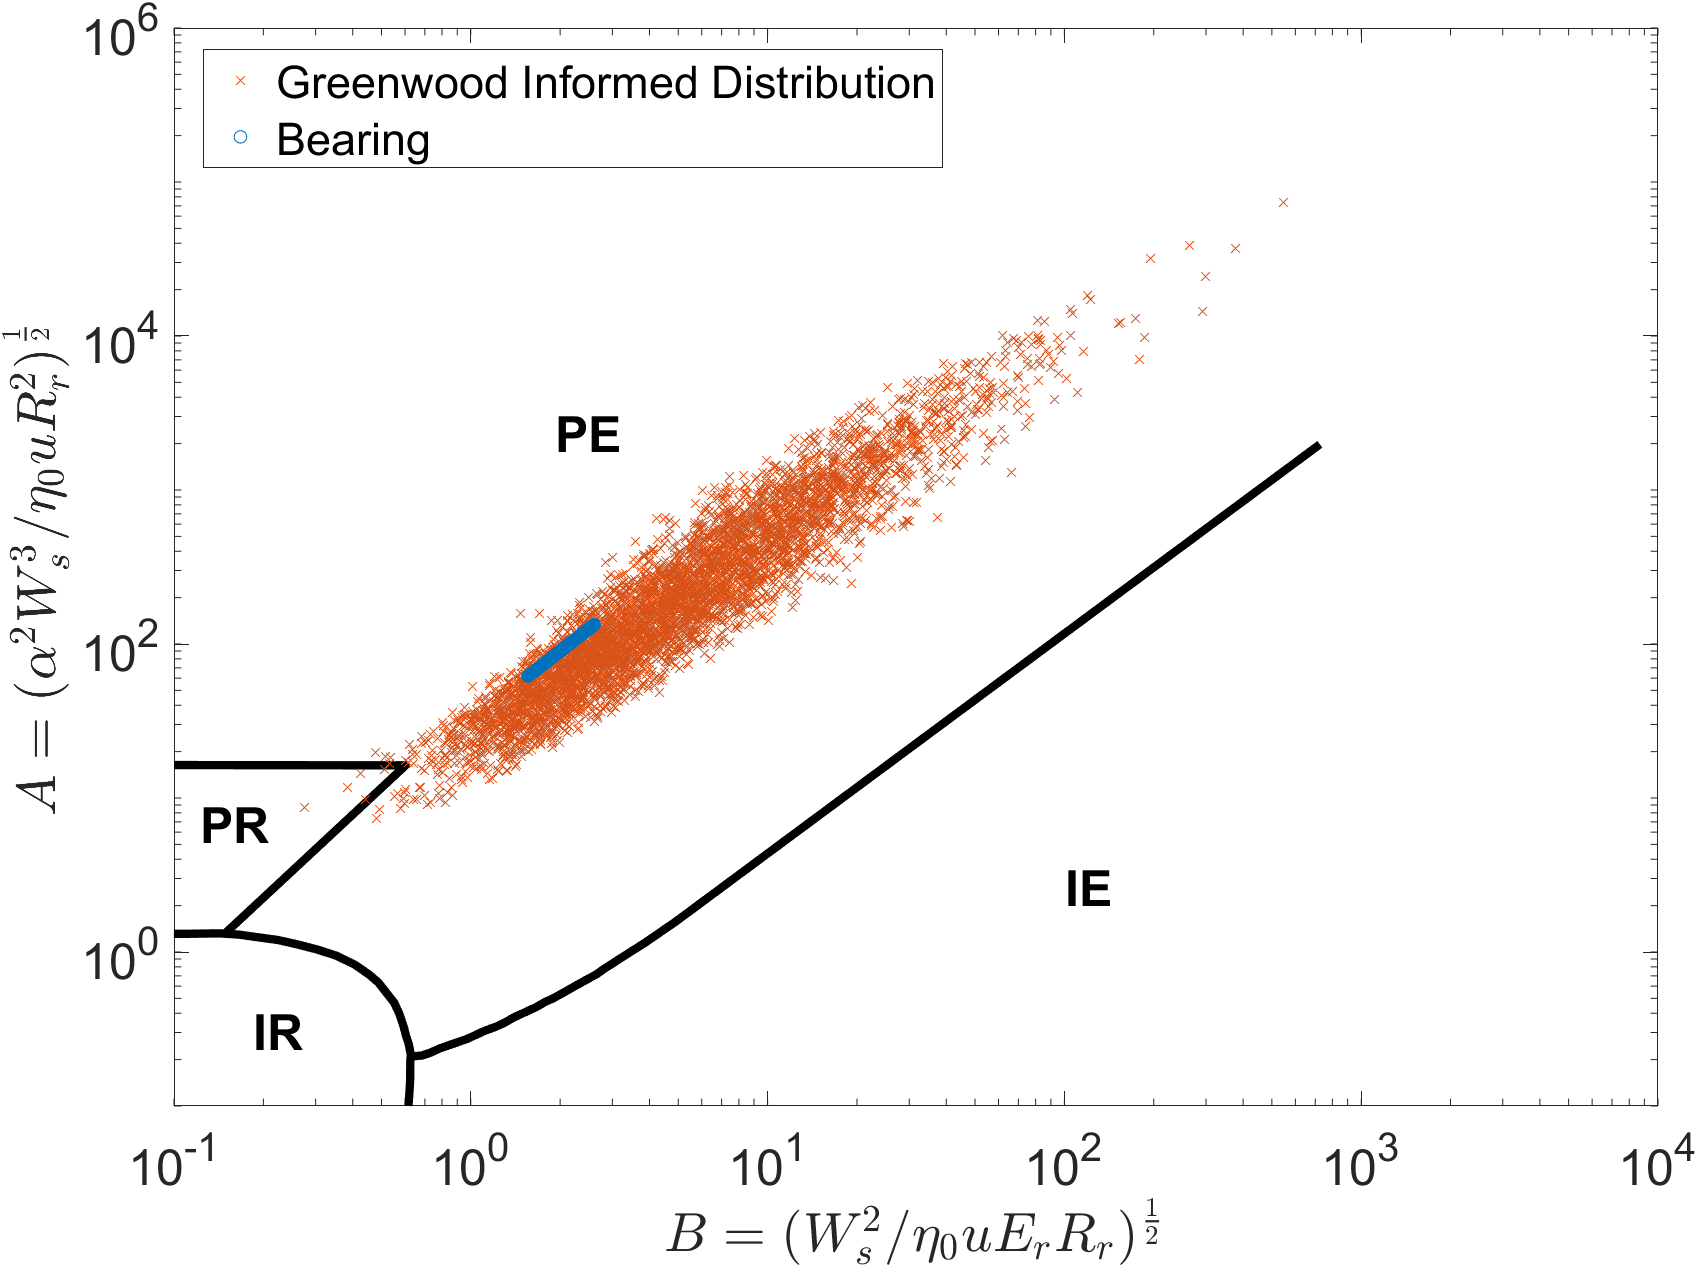
\includegraphics[width=150mm]{Greenwood_Bearing.png}
	\caption{Bearing operating conditions vs Greenwood informed training data.}
	\label{Greenwood_Bearing}
\end{figure} 


The dynamic model was run explictly as a dry model, without the influence of the EHL film at the roller-race contacts. The kinematic and dynamic results required for input to the ANN are then extracted at each time step. Results were generated for an individual element completing one complete orbit around the bearing. Extracted results include roller load per unit length, reduced radius of the contact between the roller and inner-race, and the contact entrainment velocity.

The loading pattern is cyclic in nature as the roller enters and exits the most highly loaded region of the bearing, corresponding to the force vector applied to the inner race. Sufficient preload ensures constant contact between elements and raceways so that the regime does not deviate from EHL. The contact reduced radius and entrainment speed do not change throughout the orbit as they are a function of bearing geometry and constant operating speed.

\begin{figure}
	\centering
	\begin{subfigure}[b]{0.9\textwidth}
		\centering
		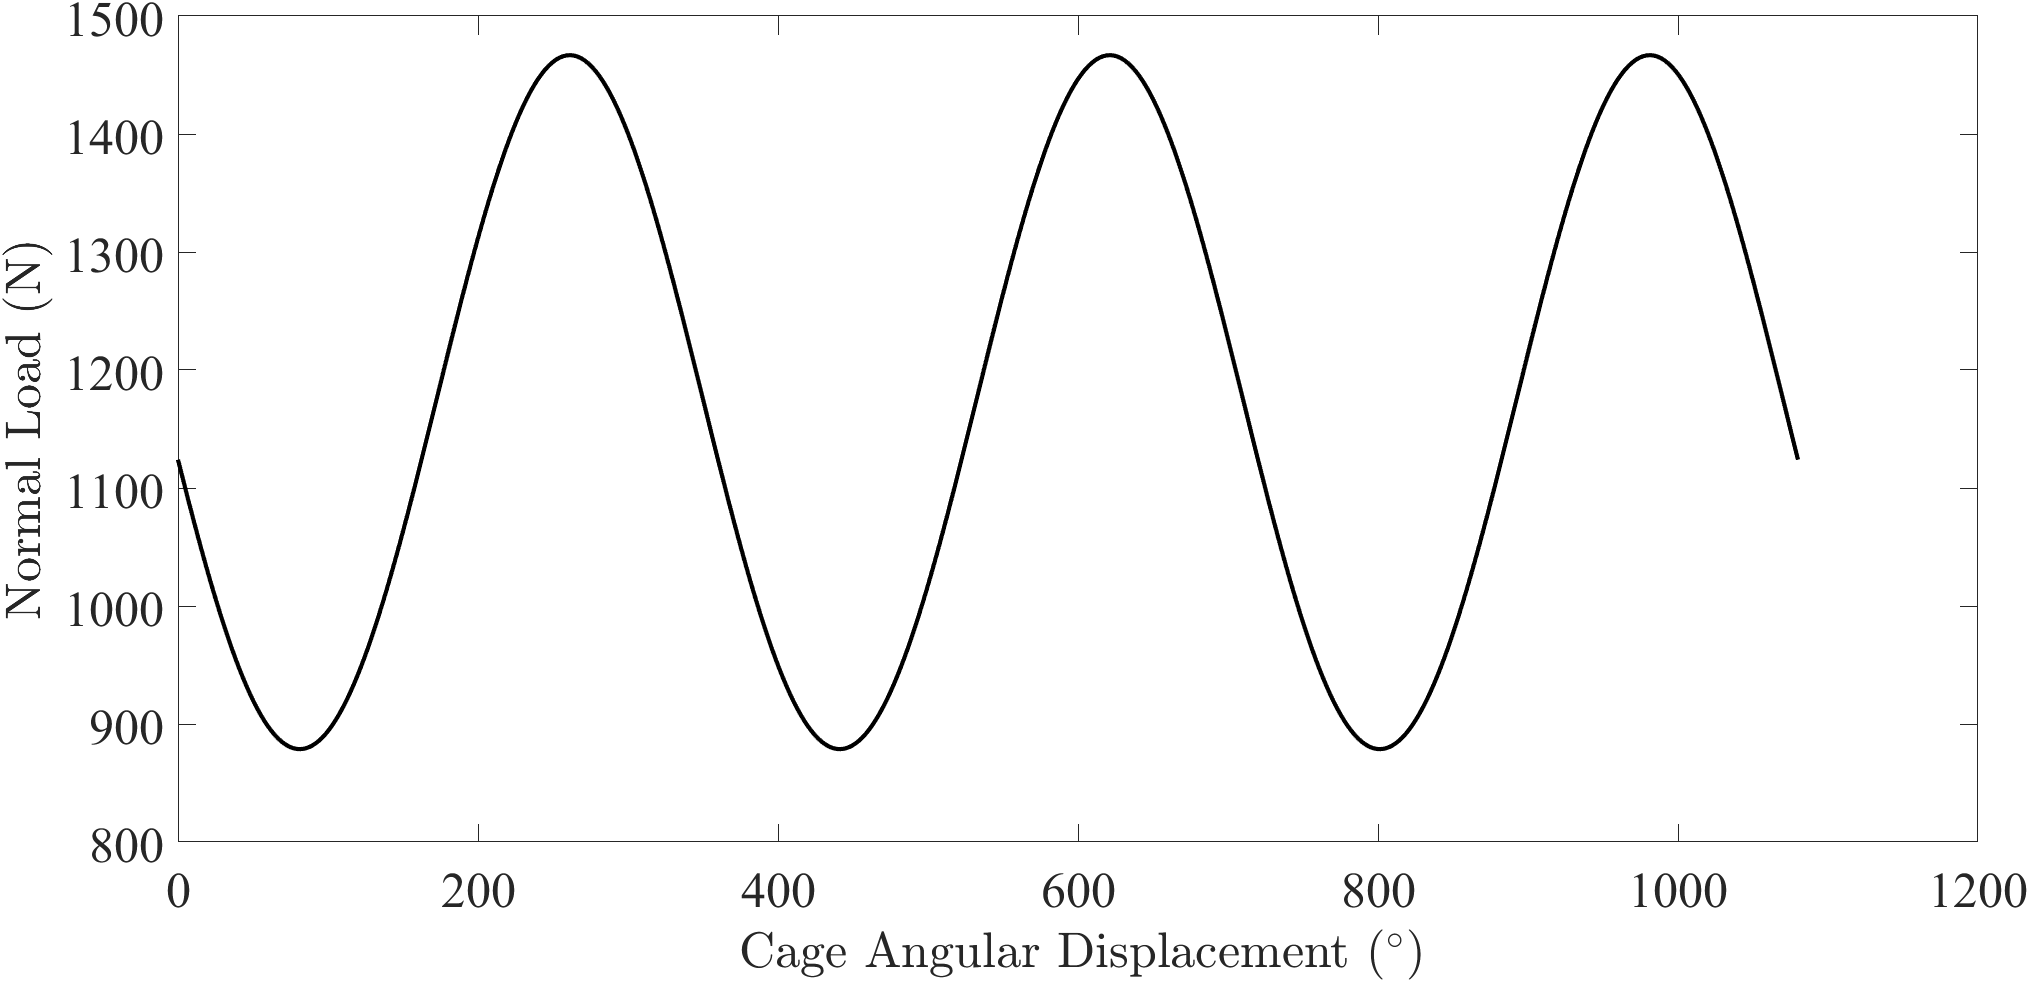
\includegraphics[width=\textwidth]{ANN_Explicit_Bearing Normal Load.png}
		\caption{}
		\label{Contact Normal Load ANN}
	\end{subfigure}
	\hfill
	\begin{subfigure}[b]{0.9\textwidth}
		\centering
		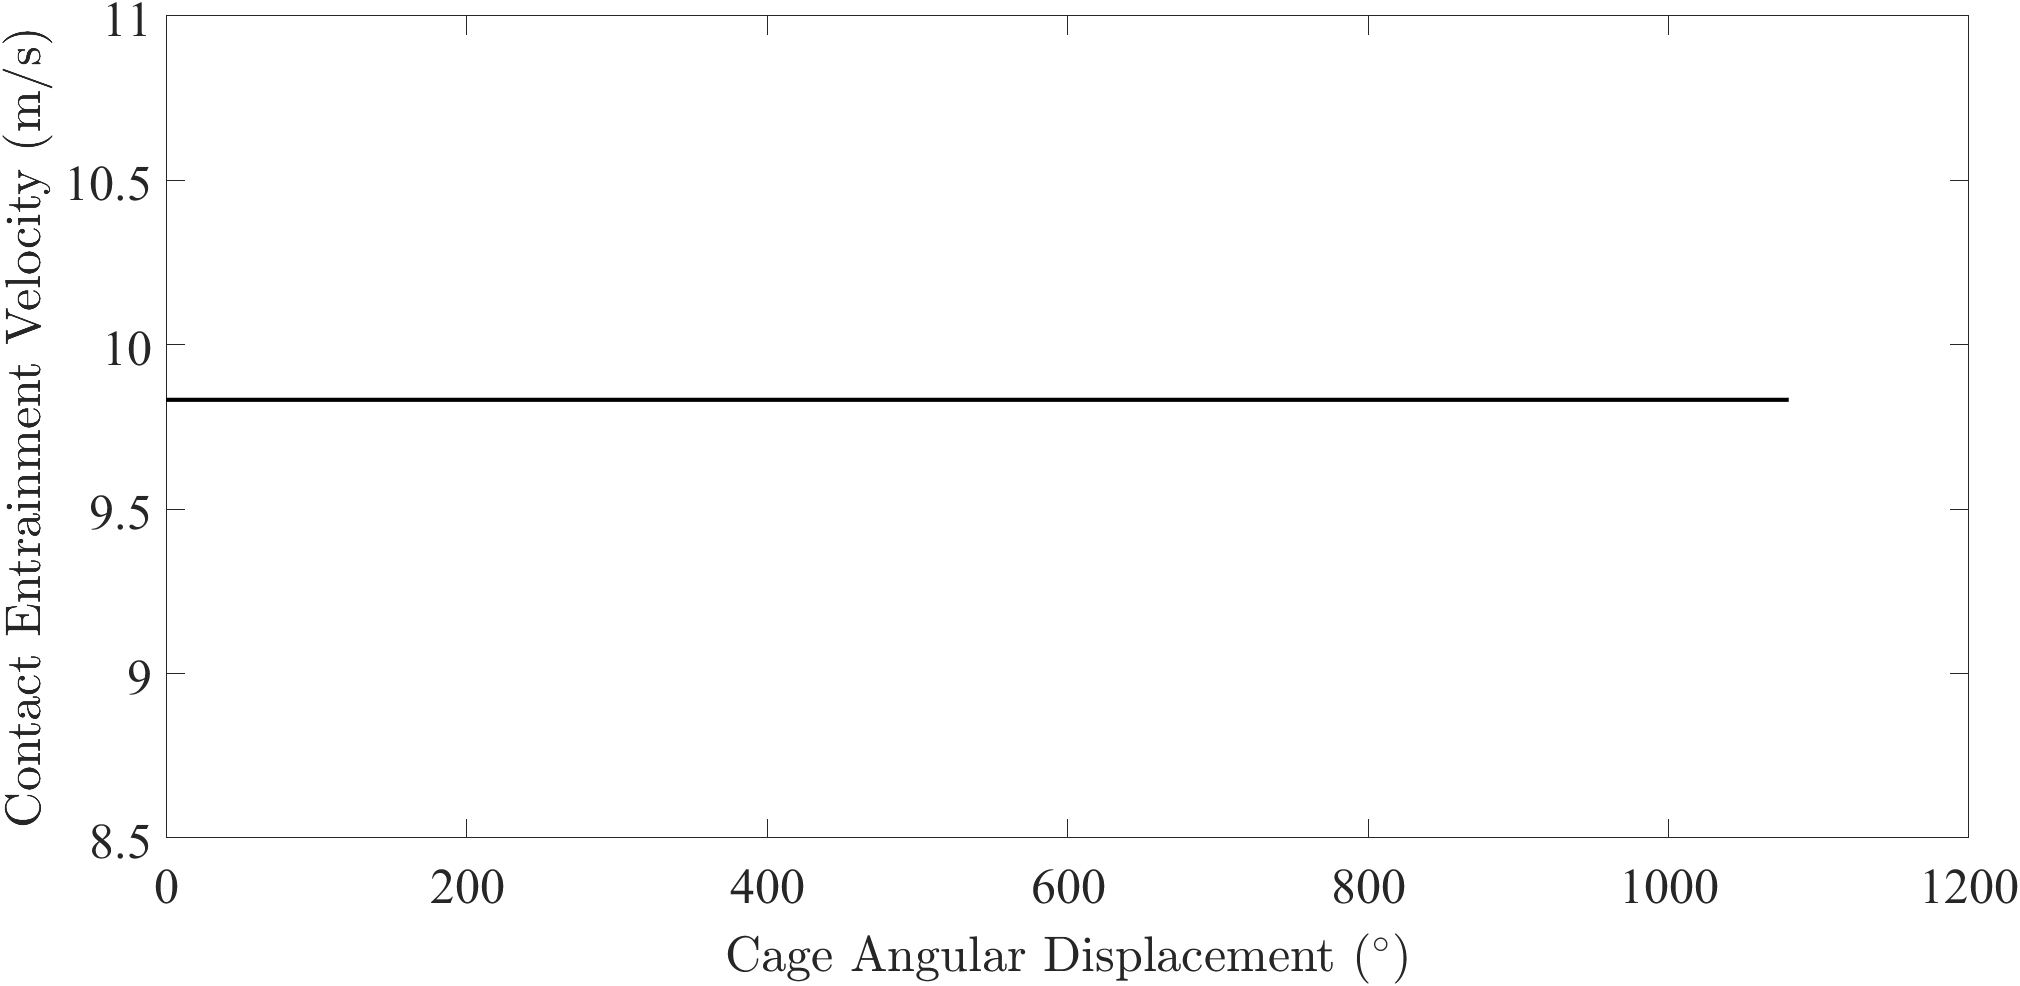
\includegraphics[width=\textwidth]{ANN_Explicit_Bearing Entrainment Velocity.png}
		\caption{}
		\label{Contact Entrainment ANN}
	\end{subfigure}
	\hfill
	\begin{subfigure}[b]{0.9\textwidth}
		\centering
		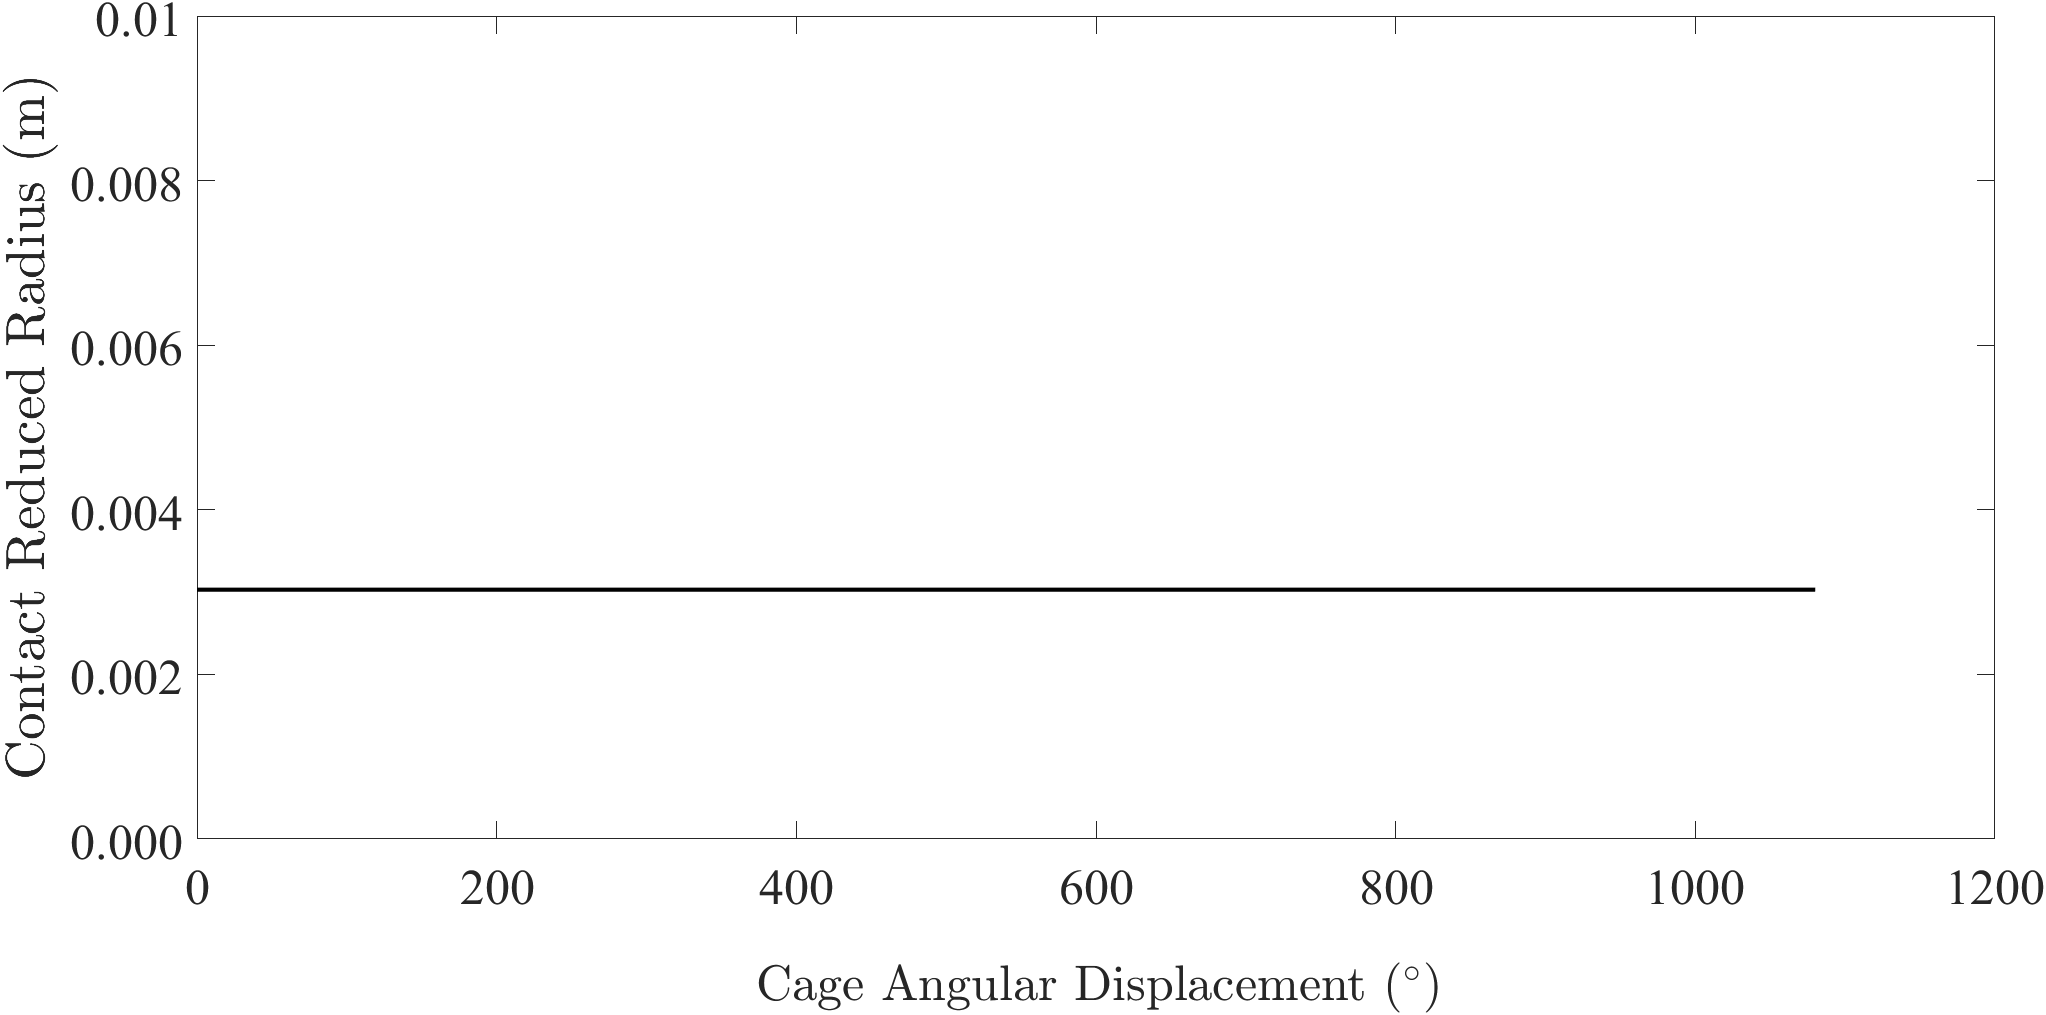
\includegraphics[width=\textwidth]{ANN_Explicit_Bearing Reduced Radius.png}
		\caption{}
		\label{Contact Reduced Radius ANN}
	\end{subfigure}
	\caption{Individual rolling element input values to ANN : a) Contact load, b) Contact entrainment velocity, c) Contact reduced radius}
	\label{Individual rolling element input values to ANN}
\end{figure}

The chosen structure and trained ANN would be used to predict film thickness across...


\subsection{Implicit Bearing Film Thickness Predictions}

Same model as in Section \ref{System level flexible model}



\section{Results and Discussion}

The following data was obtained using consumer grade hardware with the following specifications: 
Intel® Core™ i7-9750H CPU 6 cores @ 2.60GHz, 32GB RAM; GPU: NVDIA GeForce GTX 1650.

The same hardware was used for both the full numerical and the ANN solutions to provide performance comparisons and assess the suitability of ANNs for film thickness calculations in FMBD solvers.

\subsection{ANN Structure Evaluation}

The 1D EHL model presented in Section \ref{1D EHL Model} was used to generate the numerical database for training the ANN. Each numerical solution and hence training point took an average of 5.88~$s$. The construction of the entire database on a single core therefore has a wall time of between 58.8~$min$ and 489~$min$ for 600 and 5000 points respectively. This wall time is purely for baseline comparisons, and can be significantly improved using parallelisation across multiple cores.

Tables \ref{LogSig_table}-\ref{ANN_Explicit_LogSig_5000_table} present the $R^2$ values obtained from 600 data points, considering different activation functions, number of layers, and neurons. Among the activation functions tested, the ReLU function consistently underperformed when compared to the logistic sigmoid and hyperbolic tangent functions across all network structures. It is important to acknowledge that there is a slight variability in the performance of the network with each new training session. However, it is worth noting that the optimum number of layers, similar to tribological applications of ANNs \cite{Marian2021}, was found to be between two and three.


\begin{table}
	\caption{$R^2$ performance of ANN structures using 600 data points and a LogSig activation function}
	\label{LogSig_table}
	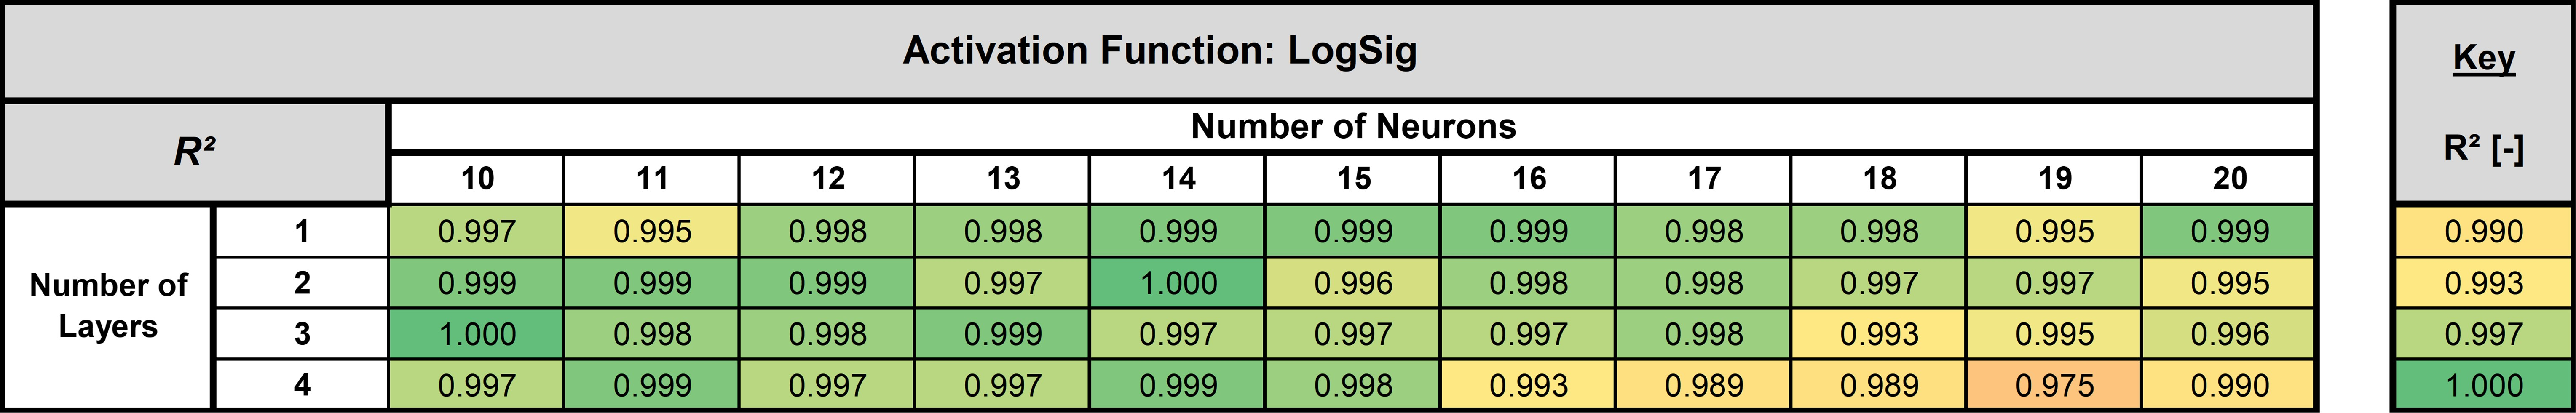
\includegraphics[width=\linewidth]{ANN_Explicit_ActFun_LogSig.jpg}
\end{table}

\begin{table}
	\caption{$R^2$ performance of ANN structures using 600 data points and a Tanh activation function}
	\label{Tanh_table}
	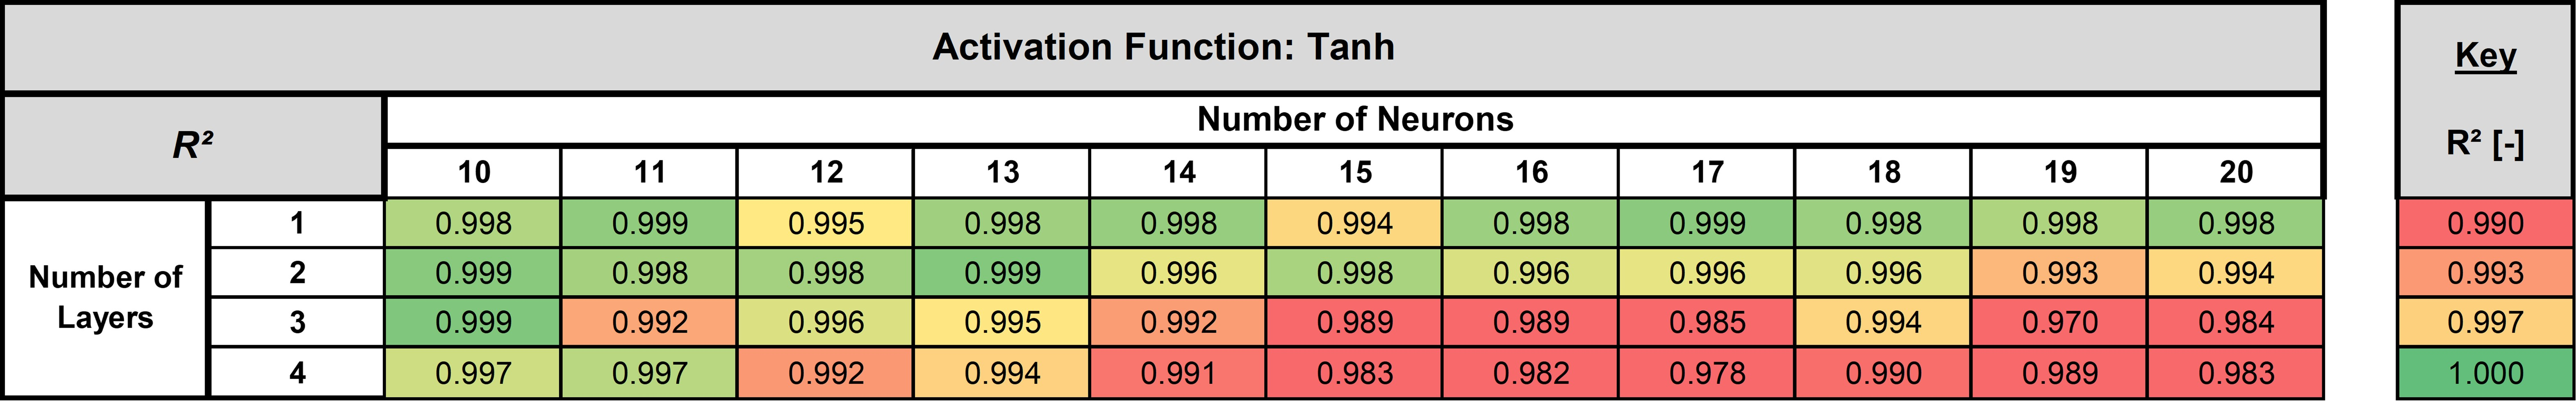
\includegraphics[width=\linewidth]{ANN_Explicit_ActFun_Tanh.jpg}
\end{table}

\begin{table}
	\caption{$R^2$ performance of ANN structures using 600 data points and a Tanh activation function}
	\label{ReLU_table}
	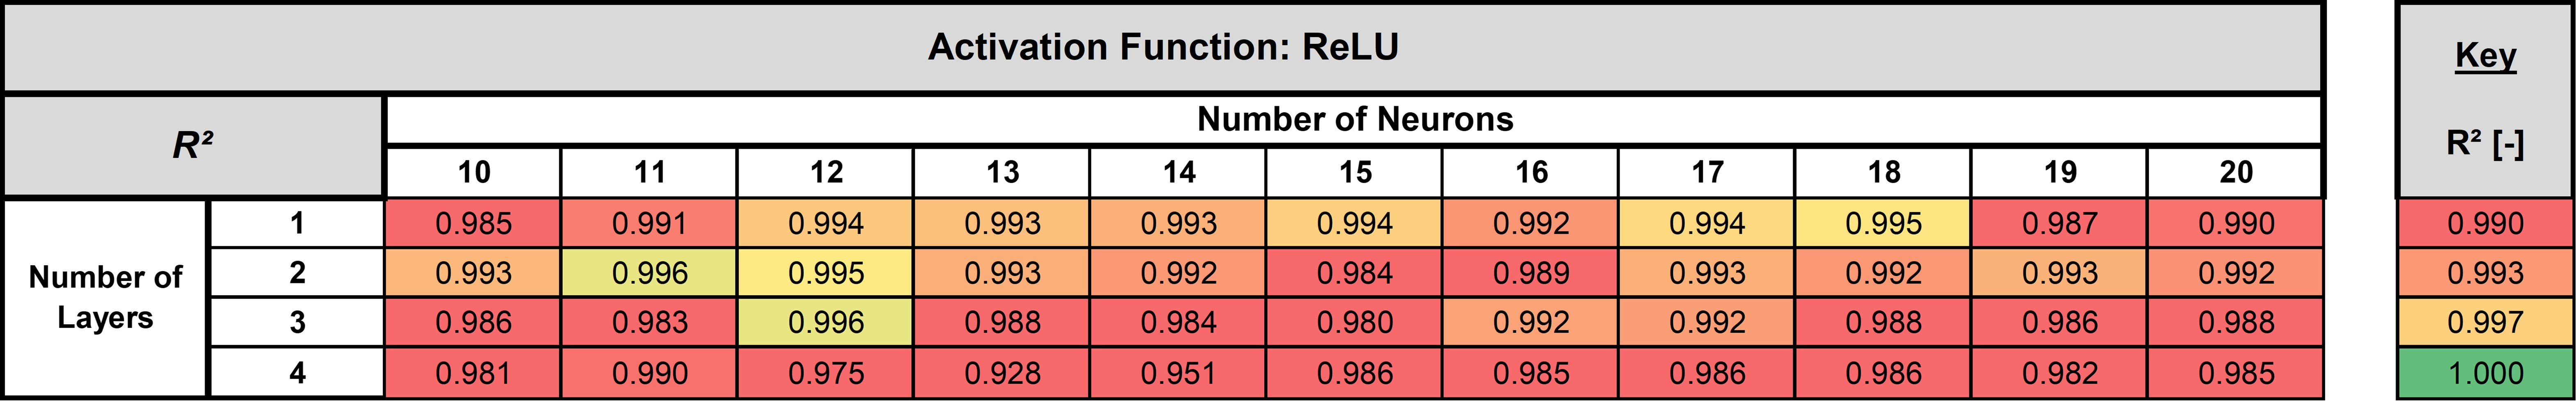
\includegraphics[width=\linewidth]{ANN_Explicit_ActFun_ReLU.jpg}
\end{table}

\begin{table}
	\caption{Training time of ANN structures with LogSig activation function and 600 data points}
	\label{ANN_Explicit_LogSig_600_table}
	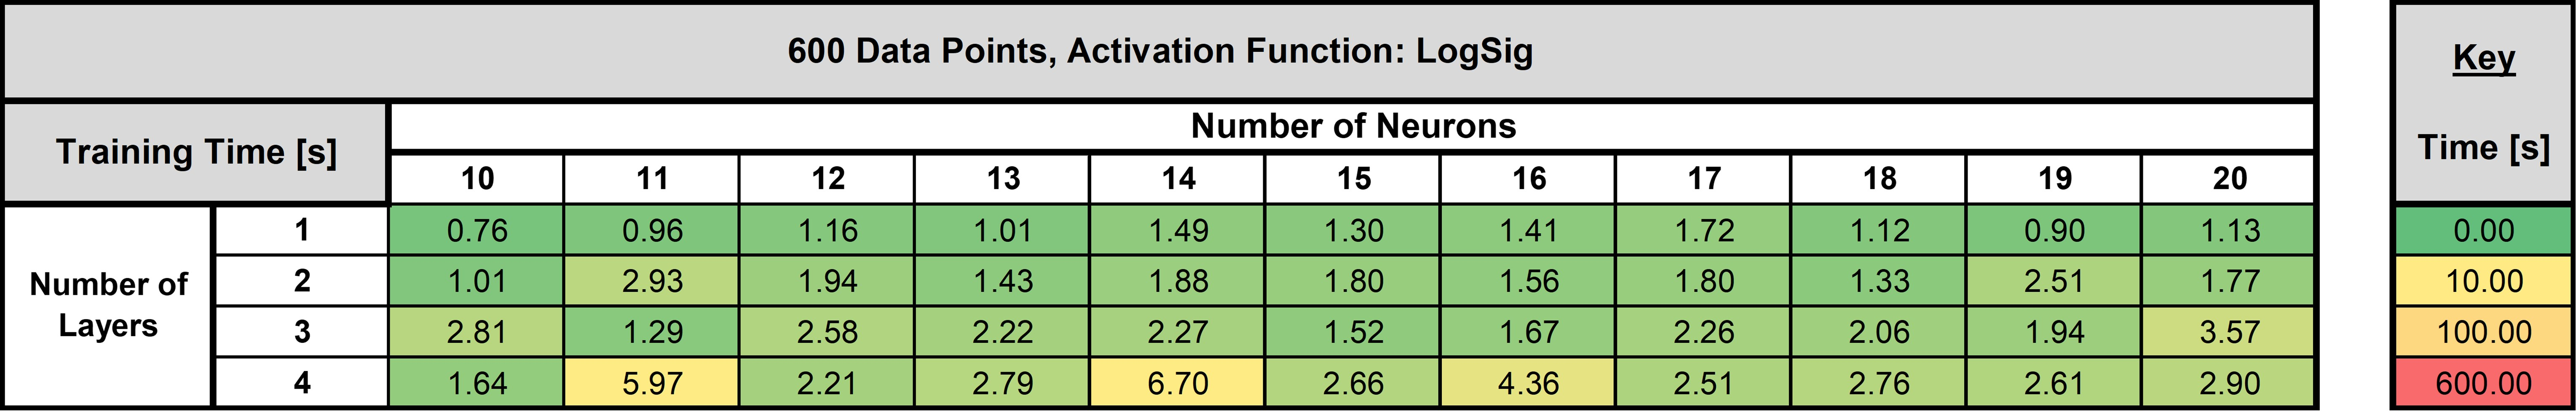
\includegraphics[width=\linewidth]{ANN_Explicit_LogSig_600.jpg}
\end{table}

\begin{table}
	\caption{Training time of ANN structures with LogSig activation function and 1000 data points}
	\label{ANN_Explicit_LogSig_1000_table}
	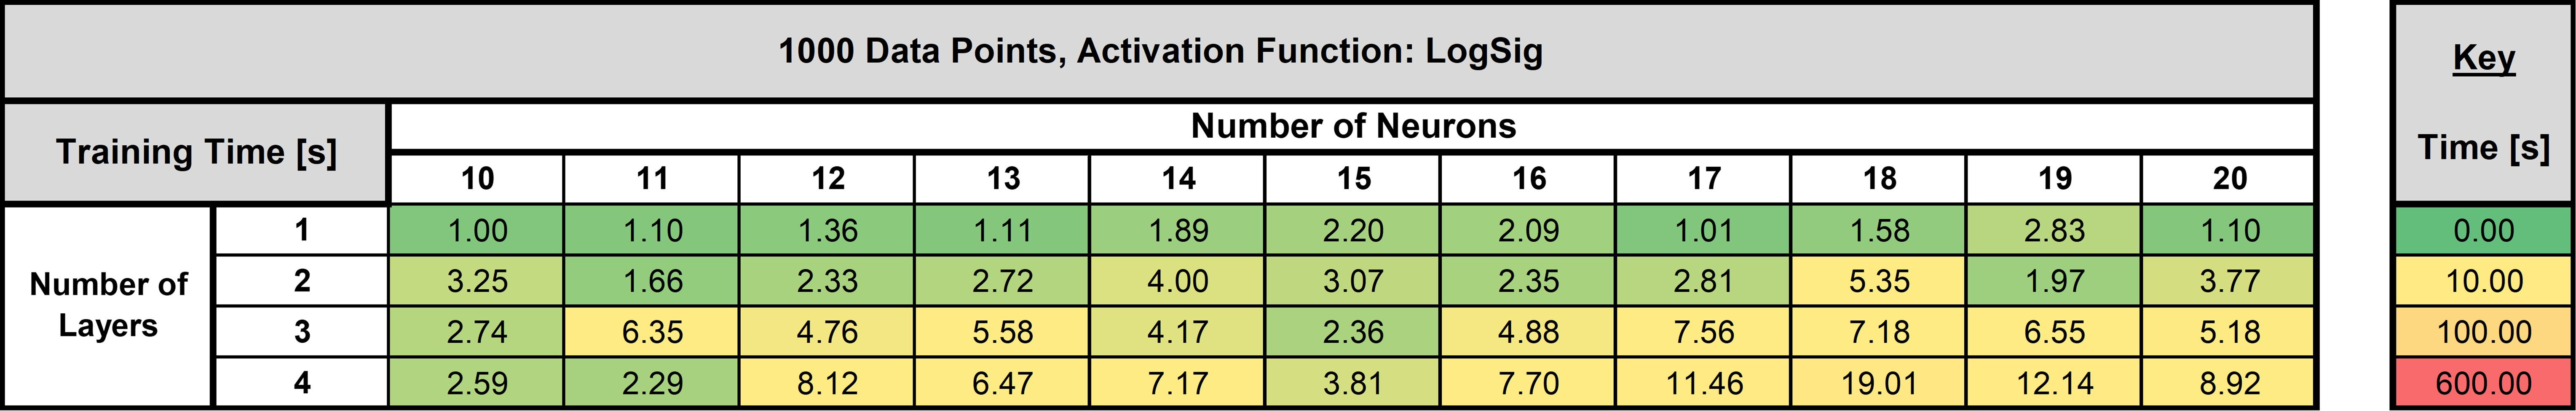
\includegraphics[width=\linewidth]{ANN_Explicit_LogSig_1000.jpg}
\end{table}

\begin{table}
	\caption{Training time of ANN structures with LogSig activation function and 2000 data points}
	\label{ANN_Explicit_LogSig_2000_table}
	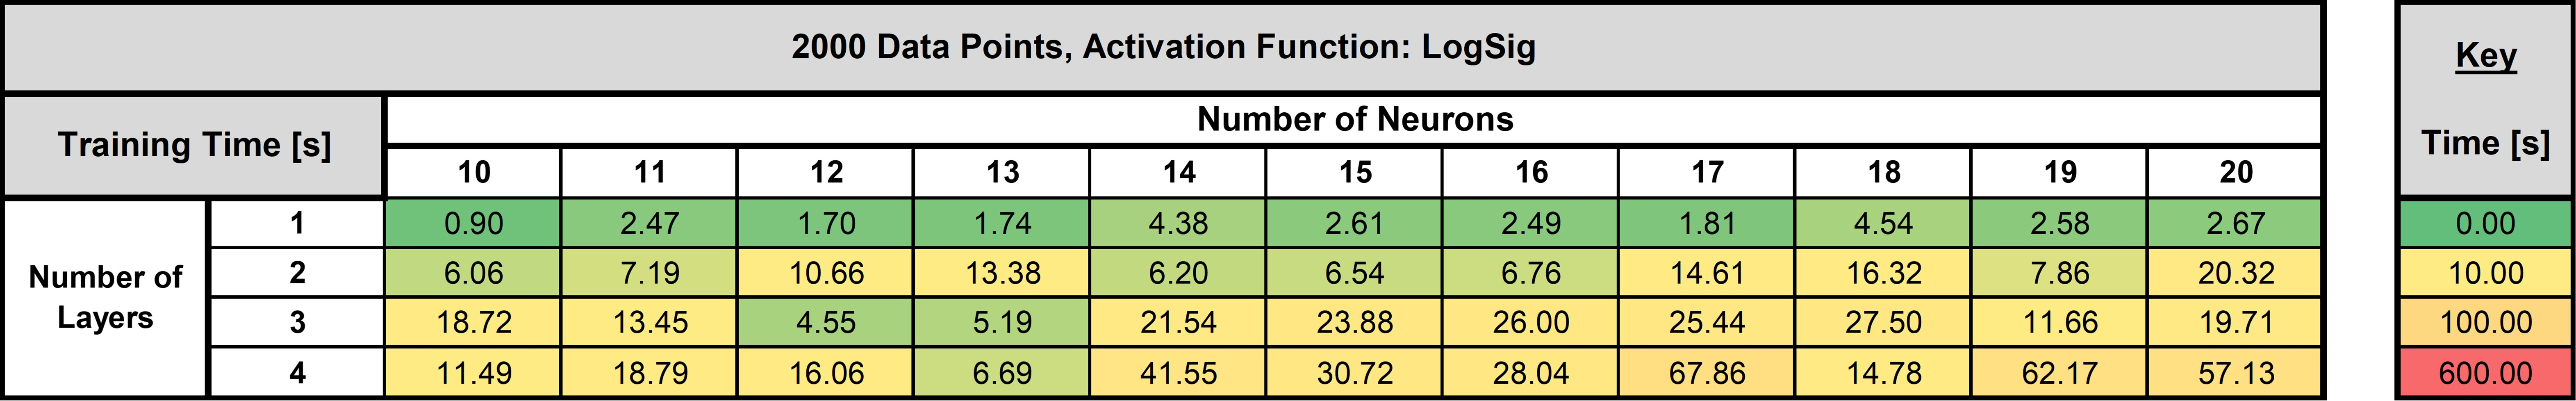
\includegraphics[width=\linewidth]{ANN_Explicit_LogSig_2000.jpg}
\end{table}

\begin{table}
	\caption{Training time of ANN structures with LogSig activation function and 5000 data points}
	\label{ANN_Explicit_LogSig_5000_table}
	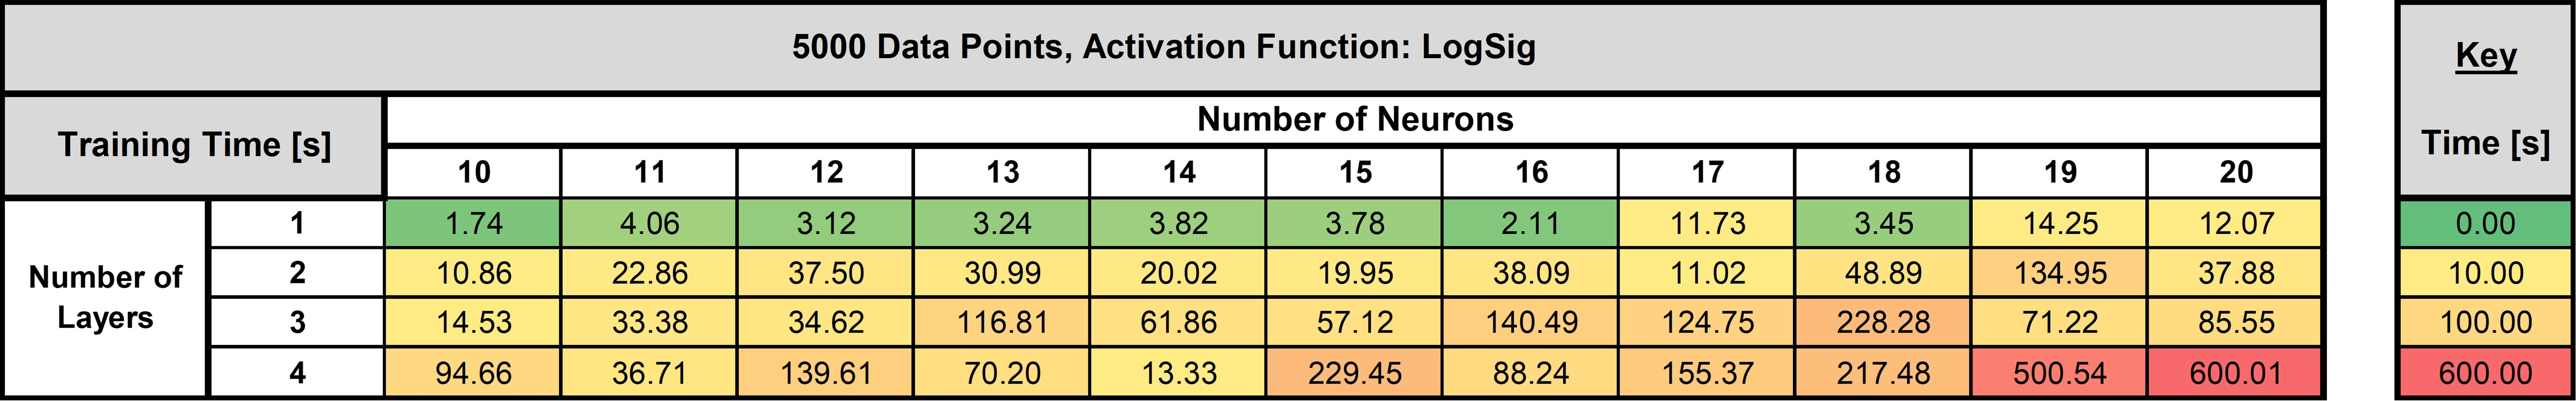
\includegraphics[width=\linewidth]{ANN_Explicit_LogSig_5000.jpg}
\end{table}

\begin{figure}
	\centering
	\begin{subfigure}[b]{0.49\textwidth}
		\centering
		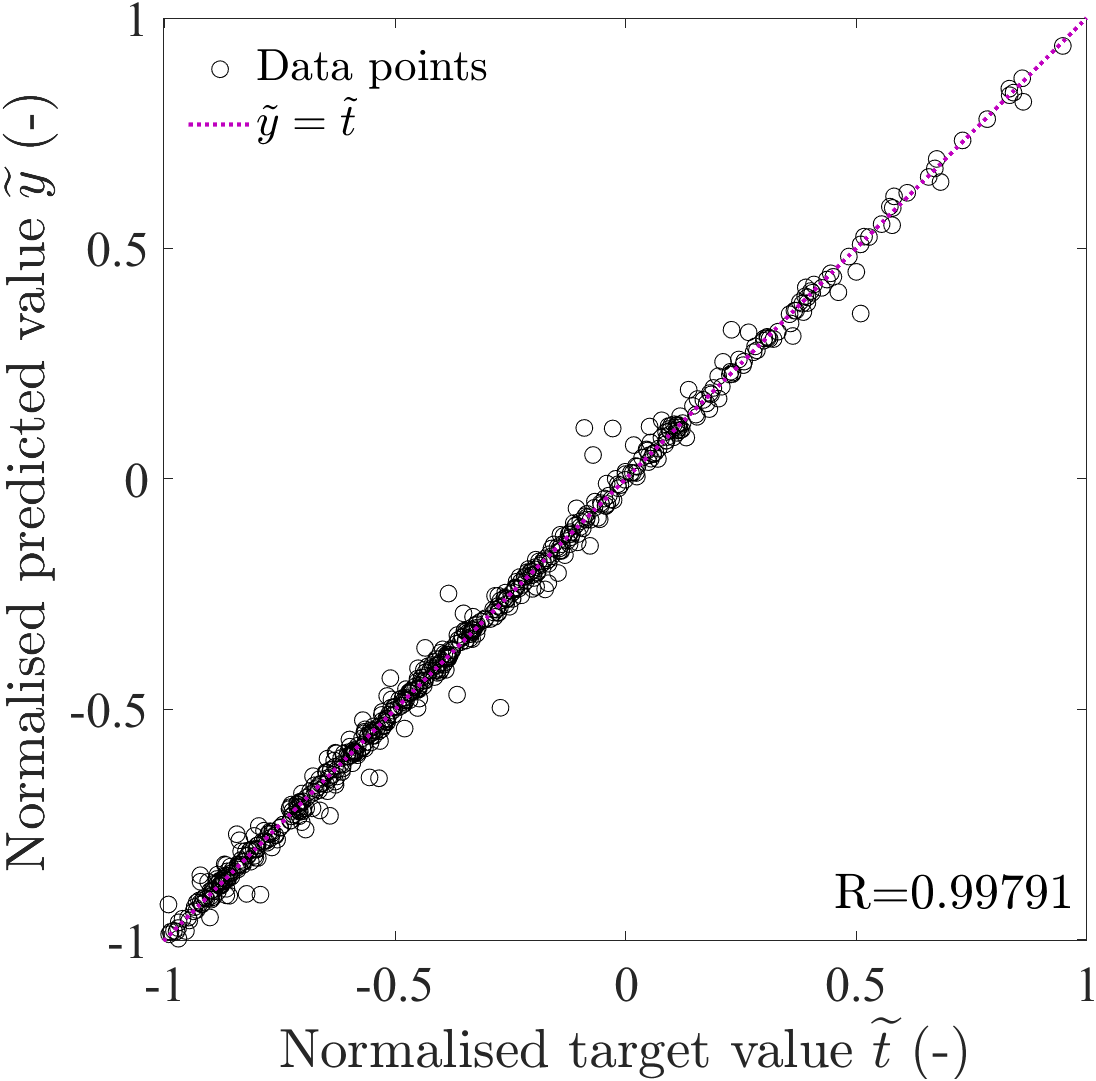
\includegraphics[width=\textwidth]{ANN_Explicit_600_Rval.png}
		\caption{}
		\label{600_Rval}
	\end{subfigure}
	\hfill
	\begin{subfigure}[b]{0.49\textwidth}
		\centering
		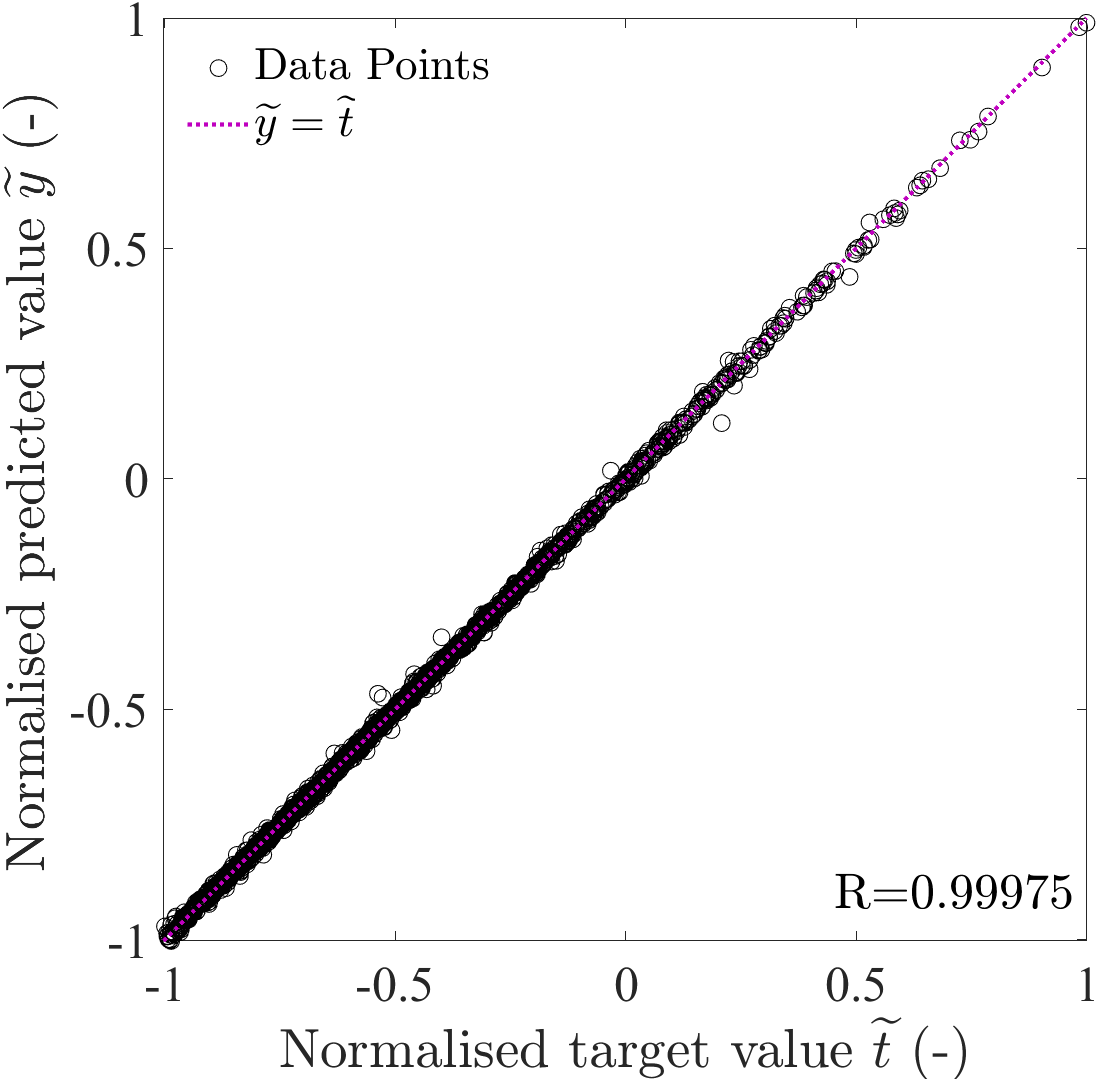
\includegraphics[width=\textwidth]{ANN_Explicit_1000_Rval.png}
		\caption{}
		\label{1000_Rval}
	\end{subfigure}
	\hfill
	\begin{subfigure}[b]{0.49\textwidth}
		\centering
		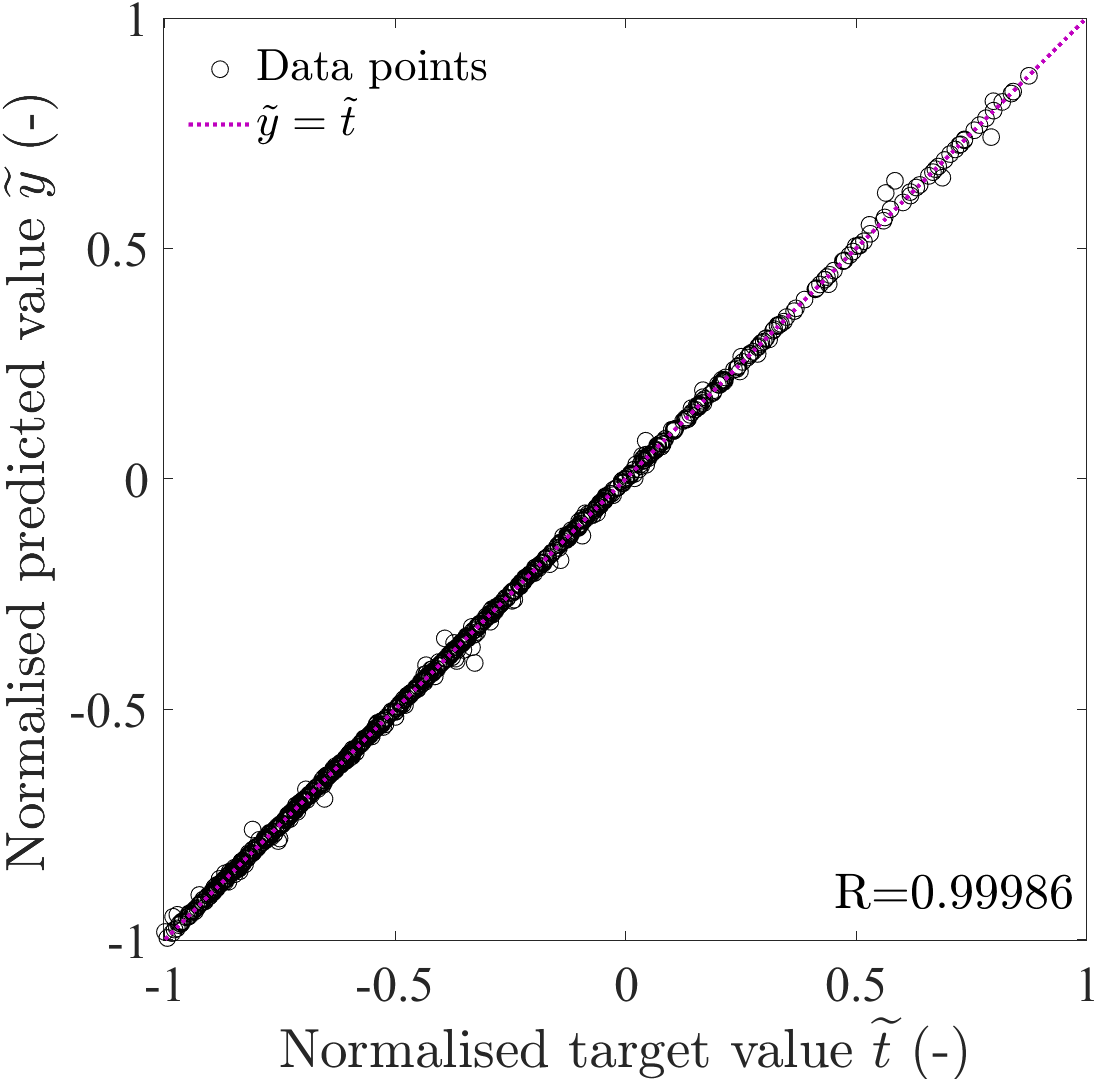
\includegraphics[width=\textwidth]{ANN_Explicit_2000_Rval.png}
		\caption{}
		\label{2000_Rval}
	\end{subfigure}
	\hfill
	\begin{subfigure}[b]{0.49\textwidth}
		\centering
		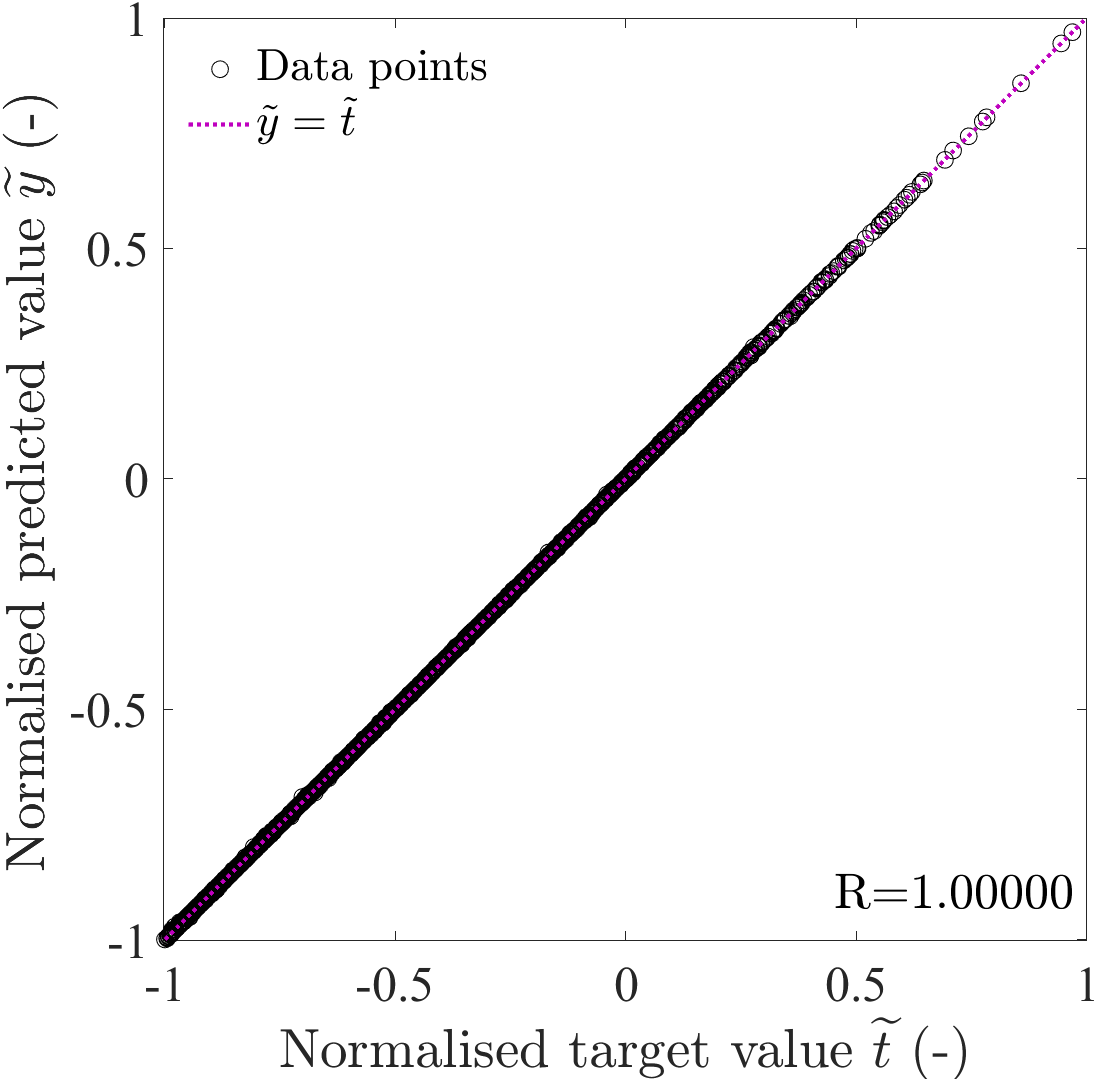
\includegraphics[width=\textwidth]{ANN_Explicit_5000_Rval.png}
		\caption{}
		\label{5000_Rval}
	\end{subfigure}
	\caption{$10-[14-14-14]_3-1$ using a Logistic Sigmoid activation function : a) 600 points, b) 1000 points, c) 2000 points, d) 5000 points}
	\label{$R^2$ performance of ANN structure}
\end{figure}







\subsection{Explicit Bearing Film Thickness Predictions}

After identifying suitable data set size and ANN structure, the ANN could then be compared to the analytical (Eq. \ref{DowsonToyodaCentralFilm}) and numerical (Section \ref{1D EHL Model}) methods of obtaining central film thickness at the roller-race contact. The operating conditions of the bearing were within the range of validity of the training data set. This is demonstrated in Figure \ref whereby the Greenwood parameters for the bearing operating points are overlayed on the training cloud.



\begin{figure}
	\centering
	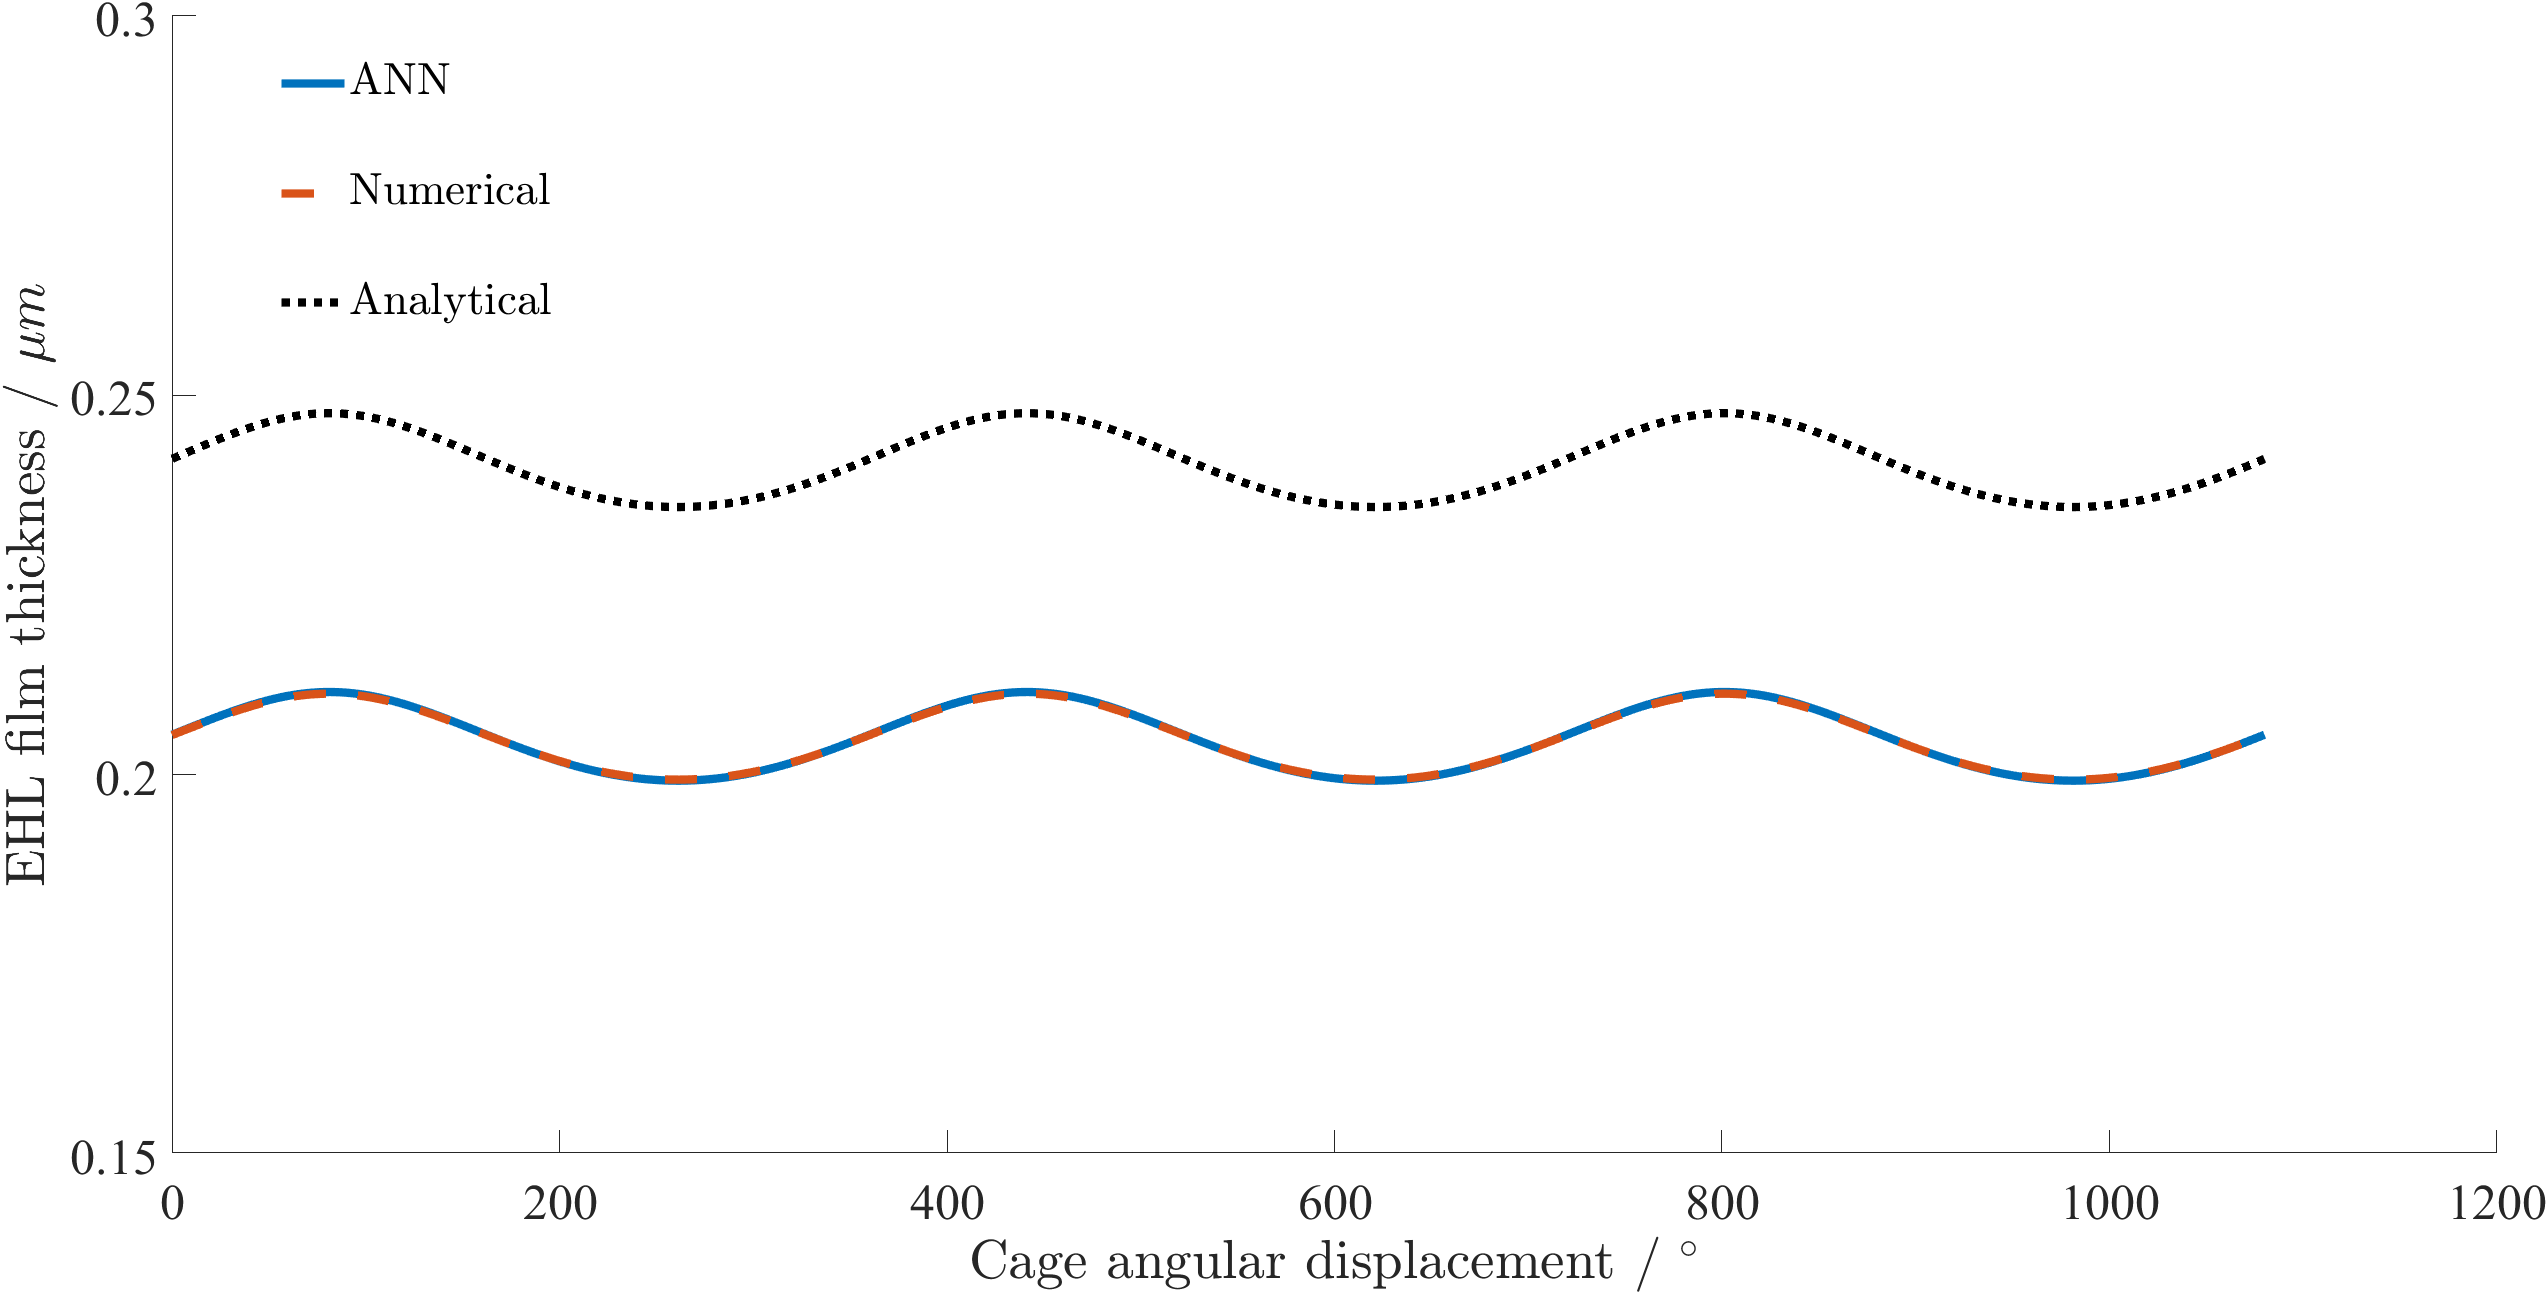
\includegraphics[width=150mm]{ANN_Explicit Film Thickness Comparisons.png}
	\caption{ANN, numerical and analytical central film thickness comparisons.}
	\label{ANN Film Thickness Comparisons}
\end{figure}
Figure 

Three different methods of obtaining the EHL film thickness were tested

\begin{table*}
	\caption{Film thickness computation methodology performance relative to the numerical solution}
	\label{Explicit time and MSE}
	\centering
	\renewcommand{\arraystretch}{1.5}%
	\begin{tabular}{|c|c|c|}
	
		\hline \multirow{2}{*}{Method} & Time per point & MSE \\
		\cline{2-3} & [$\mathrm{s}$] & [$\mu \mathrm{m}$] \\
		\hline Numerical & $4.87 \mathrm{E}+00$ & - \\
		\hline Analytical & $4.43 \mathrm{E}-05$ & $1.32 \mathrm{E}-3$ \\
		\hline ANN & $3.33 \mathrm{E}-03$ & $1.46 \mathrm{E}-8$ \\
		\hline
	\end{tabular}
\end{table*}

\subsubsection{Timing}
\subsubsection{Error}

\subsection{Implicit Bearing Film Thickness Predictions}

\subsubsection{Timing}
Each computational point, including 

\subsubsection{Error}


\section{Conclusions}
Roller bearings are only one application of these ANNs. The use cases extend far beyond roller bearings, to key components in automotive, machining and other industrial applications where interactions between contiguous surfaces exist. Film thickness is a critical parameter in the determination of NVH, friction and wear.

Full numerical solution can account for film thickness profile and pressure distribution across the contact. Futhermore, 

Echávarri et al. \cite{EchavarriOtero2014} comment on the "black box" nature of ANNs. Results from intermediate calculations are lost, which is often of interest for more in-depth analysis of contact condition; film thickness and pressure distributions and temperature for example.  

The numerical solution database can also benefit from explicit parallelisation ie. use of multiple computational cores of the CPU. When using MBD solvers implicitly it is not possible to use explicit parallelisation since a particular time step is dependent on the present timestep as well as on data of the same timestep. The ANN functionality in turn can be embedded with an implicit MBD computation environment to significantly improve the computation times without the need of explicit parallelisation despite benefitting from it indirectly. 

